\documentclass{article}


%  tif you need to pass options to natbib, use, e.g.:
%     \PassOptionsToPackage{numbers, compress}{natbib}
% before loading neurips_2023

\PassOptionsToPackage{numbers, sort&compress}{natbib}

% ready for submission
\usepackage[preprint]{neurips_2023}


% to compile a preprint version, e.g., for submission to arXiv, add the
% [preprint] option:
%     \usepackage[preprint]{neurips_2023}


% he to compile a camera-ready version, add the [final] option, e.g.:
%     \usepackage[final]{neurips_2023}


% to avoid loading the natbib package, add option nonatbib:
%    \usepackage[nonatbib]{neurips_2023}


\usepackage[utf8]{inputenc} % allow utf-8 input
\usepackage[T1]{fontenc}    % use 8-bit T1 fonts
\usepackage{hyperref}       % hyperlinks
\usepackage{url}            % simple URL typesetting
\usepackage{booktabs}       % professional-quality tables
\usepackage{amsfonts}       % blackboard math symbols
\usepackage{nicefrac}       % compact symbols for 1/2, etc.
\usepackage{microtype}      % microtypography
\usepackage{xcolor}         % colors
\usepackage{graphicx}
\usepackage{amsmath}
\usepackage{amssymb}
\usepackage{algorithm}
\usepackage{algpseudocode}
\usepackage{caption}
\usepackage{subcaption}
\usepackage{multirow}
\usepackage{rotating}

%\usepackage[fontsize=12pt]{fontsize}

\usepackage{setspace}
%\doublespacing % Or use
%\linespread{2.0}
\linespread{1.5}


\graphicspath{ {./figures/} }  %Path relative to the .tex file containing the \includegraphics command
\bibliographystyle{abbrvnat}

% New command definitions
\newcommand{\argmin}{\mathop{\mathrm{argmin}}}
\newcommand{\pluseq}{\mathrel{+}=}
\newcommand\Set[2]{\{\,#1\mid#2\,\}}

\newcommand\HWG[1]{ {\color{blue}#1} }

\DeclareMathOperator*{\argmax}{argmax}


\title{AlphaRouter: Bridging the Gap Between Reinforcement Learning and Optimization for Vehicle Routing with Monte Carlo Tree Searches}


% The \author macro works with any number of authors. There are two commands
% used to separate the names and addresses of multiple authors: \And and \AND.
%
% Using \And between authors leaves it to LaTeX to determine where to break the
% lines. Using \AND forces a line break at that point. So, if LaTeX puts 3 of 4
% authors' names on the first line, and the last on the second line, Try using
% \AND instead of \And before the third author name.


\author{%
  Won-Jun Kim \\
  Department of Future Mobility\\
  Hanyang University\\
  Seoul, Replic of Korea \\
  \texttt{glistering96@hanyang.ac.kr} \\   \\
   Kichun Lee\thanks{corresponding author} \\
  Department of Industrial Engineering\\
  Hanyang University\\
  Seoul, Replic of Korea \\
   \texttt{skylee@hanyang.ac.kr} \\
  % examples of more authors
  % \And
  % Coauthor \\
  % Affiliation \\
  % Address \\
  % \texttt{email} \\
  % \AND
  % Coauthor \\
  % Affiliation \\
  % Address \\
  % \texttt{email} \\
  % \And
  % Coauthor \\
  % Affiliation \\
  % Address \\
  % \texttt{email} \\
  % \And
  % Coauthor \\
  % Affiliation \\
  % Address \\
  % \texttt{email} \\
}


\begin{document}


\maketitle


\begin{abstract}
Deep reinforcement learning (DRL) as routing problem solvers have shown promising results in recent studies. However, a gap between computationally-driven DRL and optimization-based heuristics exists. While a DRL algorithm for a certain problem is able to solve several similar-kind problem instances, traditional optimization algorithms focus on optimizing one specific problem instance. In this paper, we propose an approach, AlphaRouter, which bridges the gap between reinforcement learning and optimization for solving routing problems. Fitting to routing problems, our approach first proposes attention-enabled policy and value networks consisting of a policy network that produces a probability distribution over all possible nodes and a value network that produces the expected distance from any given state. We modify a Monte Carlo tree search (MCTS) for the routing problems, selectively combining it with the routing problems.  Our experiments demonstrate that the combined approach is promising in yielding better solutions compared to original RL approaches without MCTS and good performance comparable to classical heuristics.
\end{abstract}


\section{Introduction}

In NP-hard combinatorial optimization (CO) problems, finding global optimum solutions is computationally infeasible. Instead of finding global optima, numerous heuristics showed promising results. Despite the high effectiveness of heuristics, their application in real-life industries is often hindered by a variety of problems and uncertain information.
Indeed, the heuristics, mathematically originated, are dependent on problem formulations for their proper application. However,
an exact formulation of constraints is quite challenging in reality
as some constraints are rapidly changing and highly stochastic even in a distributional sense.
For instance, a few constraints vanish at a time and other constraints newly enter with coefficients that, being unknown, should be estimated by an assumed distribution and a certain procedure.
As real-life domains are entangled with various participants and requirements, some constraints are too complex to formulate.
In such situations, thus, particularly when simulation is possible as in a game, the approach of RL has recently attracted attention in the literature and industry.


%is difficult as some rapidly changing constraints prevent the usage of already-made heuristics, which are fitted to the situation without newly introduced constraints. Especially, as the industry is entangled with various participants along different domains, the constraints are more complex to carefully formulate.

Mostly, the heuristics aim to solve one specific problem. That is to say, heuristics made for capacitated vehicle routing problems (CVRP), for example, cannot apply to bin-packing problems. To deal with versatile constraints and complex problems, the use of deep neural network architectures coupled with RL, called as DRL, has recently been considered effective
\cite{kwonMatNet, kwonPOMOPolicyOptimization2021}. The DRL approach is flexible as translating a problem into a reinforcement learning framework is straightforward without necessiating mathematical solutions but by  appropriately defining both state and reward and running computational simulations.
In the long run, the ultimate goal of the DRL approach is to find a new and computational way to solve a complex problem that surpasses the performance of mathematically exact algorithms and their heuristics \cite{tensor_mult_RL}.


Nonetheless, the current stage of DRL's performance is not statisfactory enough to reach the performance of heuristic solvers, and is still on the journey to the ultimate goal. Our work is to improve DRL performance by attempting to reduce the gap between heuristic solvers and DRL. Motivated by the AlphaGo series \citep{silverMasteringGameGo2016, silverMasteringGameGo2017, schrittwieserMasteringAtariGo2020}, we propose a deep-layered network for RL equipped with selective application of a Monte Carlo Tree Search (MCTS), a general framework applicable to various types of CO problems. We modify some components of MCTS for the application to routing domains that are different from a game.
Unlike the AlphaGo series, we found that a mere application of the MCTS to every action choice is inefficient, thereby proposing a selective application of our MCTS for routing problems.
In this paper, the domain is routing problems that will be extensible to other problems.

Indeed, the neural network architectures have been introduced before in RL contexts \cite{kool2018attention, daiLearningCombinatorialOptimization2018, kwonPOMOPolicyOptimization2021}. However, to the best knowledge of ours, no attempt has been made to improve network architectures for routing problems integrated with customized MCTS.
The introduced RL framework is quite beneficial if the resulting network is applicable to other problem types by using the same network architecture as suggested in \cite{vinyalsPointerNetworks2017, kwonPOMOPolicyOptimization2021, kwonMatNet}.
%{\color{red} XX: did you include this experiments? For this paper, I did not. However, considering how MCTS works, I believe it is applicable to other problems. Actually, MCTS was used in various Games like GO, MuJoCo(?) and other Atari Games previously with the same network.}
%{\color{blue} XX: what does this mean? -- As high-resource-demanding algorithms prohibit one from actually trying and testing the algorithms, the proposed framework is good in that context. --}
%This can stimulate the communication between the engineers and the operators in the field, enabling the participants to react to some changes in the problem conditions or goals.
%Routing problems are among the most well-known combinatorial optimization problems, with vehicle routing problems (VRP) and traveling salesperson problems (TSP) being the two main types. TSP aims to find a Hamiltonian path with minimum cost while VRP involves finding an optimal route for a fleet of vehicles to serve a set of customers with different demands while minimizing cost, or distance. These problems are typically addressed in the operations research and algorithm communities, with heuristics being the preferred method for finding the most near-optimal solution for a specific problem instance. For a comprehensive overview of heuristic methods in routing problems, refer to \citep{vinyalsPointerNetworks2017}.
%However, heuristic-based methods can be time-consuming, necessary to be built for each routing problem, and, therefore, not suitable to be used in real-time services. This has motivated researchers in the machine learning (ML) community to apply neural networks to solve routing problems. Because routing problems are NP-hard, obtaining true labels (or best paths as ground-truths) is computationally impossible, which has led to the widespread use of reinforcement learning (RL) involving training neural networks. RL-based approaches have demonstrated superior performance over heuristics in terms of inference time.
% Despite their success, RL-based approaches have not yet surpassed nor reached heuristic solvers' performance. We hypothesize that this is due to the RL objective function being formulated with the expectation of a reward distribution, while heuristic-based methods aim to find a solution set for a specific problem instance. To bridge this gap, we introduce AlphaRouter, a new approach of RL focusing on routing problems, combining RL with Monte Carlo Tree Search (MCTS) to improve the generality of well-constructed RL models on one specific routing problem instance. We adopt MCTS for its effectiveness in solution-search processes, inspired by the pioneering research proposed in an AlphaGo series \citep{silverMasteringGameGo2016, silverMasteringGameGo2017, schrittwieserMasteringAtariGo2020}.
The contributions of our paper are threefold: (1) We propose a deep-layered neural network architecture, fitting to the routing problem, with a policy gradient using a value network; (2) We propose a new MCTS strategy, demonstrating that the integration and selective application of our MCTS into the neural network architecture improves the solution quality; (3) We also demonstrate the effect of activation to improve the solution quality.
%\end{itemize}
In short, the main focus of this paper is to propose an effective RL architecture with a modified MCTS strategy for routing problems and to improve search performance. Notably, although we have proposed a neural network architecture specialized to routing problems, any neural network architecture containing a policy and a value, which will be described in later sections, can be integrated into MCTS \cite{schrittwieser2020mastering}.

We organize the rest of the paper as follows: In Section 2, we provide an overview of previous works related to combinatorial optimization, routing, and MCTS. In Section 3, we briefly introduce a general formulation of capacitated VRP and our problem's objective. In Section 4, we expound our proposed approach, AlphaRouter. In Section 5, we present our experimental results.

\section{Related works}

%\subsection{Routing problems}

Routing problems are among the most well-known set of problems in combinatorial optimization. A traveler salesman problem (TSP), one of the simplest routing problems, is to find the sequence of nodes with the shortest distance. On the other hand, a vehicle routing problem (VRP), similar to TSP, is a routing problem with the concept of depots and demand nodes. Numerous variants of VRP exist in the literature such as VRP with time windows and VRP with pickup and delivery among many \cite{kumarSurveyVehicleRouting2012}. In this paper, we focus on the capacitated VRP (CVRP), where a vehicle has a limit on its loading amount. Although some variants handle multiple vehicles, we only consider one vehicle for simplicity.

Traditionally, solutions for these problems mainly belong to two types: using math-based approaches like mixed integer programming or applying carefully designed heuristics for a specific type of problem. An example of the latter is the Lin-Kernighan heuristic \cite{linEffectiveHeuristicAlgorithm1973}. In fact, through the past decade, hybrid genetic searches with advanced diversity controls were introduced and applied to various CVRP variants successfully, greatly improving the computation time and performance\cite{HGS, hybridGeneticSearch_Vidal}. We agree that the current stage of DRL is hard to reach nor pass the performance of the analytically driven heuristics, but still, there should be efforts to solve the problem using less mathematics-entangled methods such as dynamic programming and stochastic optimization.

%\subsection{Neural networks for routing problems}

Recent research on neural networks for routing problems can be broadly categorized into two approaches based on the type of input they use: graph modules and sequential modules. Graph modules take a graph's adjacency matrix as an input and employ graph neural networks to solve routing problems, which are naturally suited to graph structures of routing problems \cite{daiLearningCombinatorialOptimization2018, kwonMatNet}. In contrast, sequential models use a list of node coordinates as input and are designed to be compatible with certain types of exact solution inputs. In this paper, we focus on the sequential module approach.

The pointer network \cite{vinyalsPointerNetworks2017} is the early model for solving routing problems. It suggested a supervised way to train a modified Seq2Seq (sequence-to-sequence) network \cite{sutskeverSequenceSequenceLearning2014} with an early attention mechanism \cite{luongEffectiveApproachesAttentionbased2015} by producing an output that is a pointer to the input token. However, a significant disadvantage of the pointer network is that one cannot obtain enough true labels to train large problems since routing problems are NP-hard. To overcome this limitation, the approach in \cite{belloNeuralCombinatorialOptimization2017} introduced the RL method for training neural networks using the famous and simple policy gradient theorem \cite{suttonPolicyGradientMethods}.

Similar to machine translation evolving from Seq2Seq to Transformers \cite{vaswaniAttentionAllYou2017}, routing has also adopted the Transformer architecture in the research \cite{kool2018attention} using both the attention layer to encode the relationships between nodes and the encoding in the decoder to produce a probability distribution for most promising nodes. Replacing the internal neural network only, they kept the training of RL the same as in \cite{belloNeuralCombinatorialOptimization2017}.

In addition to designing neural architectures, some works focus on the search process itself. For example, the work \cite{kwonPOMOPolicyOptimization2021} introduced a parallel in-training search process, named POMO, based on attention network designs. POMO algorithm assigns a different start node for several rollouts and executes the multiple episodes concurrently. An episode or rollout can be understood as a process in which a vehicle travels to the next customer until all customers are visited. Among the many episodes, they selected one best solution as the final solution. Although it does not introduce any more parameters to the model, the size of the input is bound to be $O\left(N^2\right)$ usually, where $N$ is the number of total nodes in the problem. Another approach is to adjust the weights of a pre-trained model during inference to fit the model into a single problem instance, as proposed in \cite{hottungEfficientActiveSearch2022}.

%\subsection{Monte Carlo Tree Search (MCTS)}

MCTS is a decision-making algorithm commonly used in games, such as chess, Go, and poker. The algorithm selects the next actions by simulating the game and updates the decision policy using data from the simulation. The original algorithm consists of four phases: selection, expansion, rollout, and backpropagation. In the selection phase, the algorithm starts at the root node and recursively goes down to a child node, maximizing upper confidence bound (UCB) scores. This score balances exploration and exploitation in the selection process by considering the visit counts and the average value (i.e., average winning rate) gained on that node. A more detailed explanation of UCB is in reference to \cite{bubeckRegretAnalysisStochastic2012}.

When the selection phase ends and the current node is a leaf node, the expansion phase is executed, in which a new child node is appended to the leaf node following a specific policy named ``expansion policy". Then, the rollout phase, using ``rollout policy", simulates the game until it ends and gathers the result (i.e., win or lose). In the backpropagation phase, by backtracking the path (sequence of selected nodes), the evaluated result from the rollout policy is updated for each node. For example, the updates are increasing visit counts by one and updating the average win rate with the result from the rollout phase. We note that there are two different policies used in the original MCTS, but in our MCTS implementation, only the expansion policy exists and the rollout policy is replaced by the value network. We describe more on this in Section 4. %\HWG{XX: why mention two different policies here?}

Since MCTS shares similarities with routing problems in that sequential decision-making involves, we have adopted MCTS as an additional search strategy for routing problems. In the game of Go, the next move is selected sequentially based on the board situation. In routing, the next node to visit is selected sequentially based on the current position and other external information, such as nodes' location and demands. Thus, the similarity between Go and routing is obvious.

Neural networks have been successfully integrated with MCTS in AlphaGo \cite{silverMasteringGameGo2016}, and AlphaGo Zero achieved even better results by introducing a self-play methodology for training the network \cite{silverMasteringGameGo2017}. The first AlphaGo used two different neural networks for ``expansion" and ``rollout" inducing a computational burden because of many recursive calls for the ``rollout" network until the end of the game. This problem is solved by AlphaGo Zero, in which one call for the value network predicts the expected result from any given state (or node). This was originally gathered in the rollout phase. In short, only one call for the value network replaced numerous calls for the rollout network, saving substantial computations. Our work adopts this idea for efficient MCTS simulation.

Some more recent works that integrated neural network with MCTS not only exists in the area of games but also in a Q-bit routing challenge \cite{QubitRouting_with_MCTS}. In the final stage of writing this paper, we have found a recent paper that utilizes a similar approach to our method but for a slightly different problem \cite{AlphaRouter_AAAI}. Using a neural network with MCTS is therefore a fine approach to solve a problem.

\section{Preliminaries}
Before expounding our work, we introduce a formulation of CVRP with one vehicle to connect with our routing problem. We notice that TSP can be easily formulated from CVRP by modifying some conditions.

We start with a set of $n$ customers, and each customer $i$, $i=1, \cdots, n$, has a predefined positive demand quantity $q_i$. To fulfill the customers' demands, the vehicle starts its route at the depot node, indexed as $0$. The vehicle must visit each customer only once, and its capacity cannot be more than $Q^{max}$. In conventional settings, assumably , $Q^{max}$ is set to be sufficiently large to fulfill all customers' demand. However, in practice, a vehicle may start with small $Q^{max}$ due to lack of information and its load should be refilled. We observe that the problem formulation itself below cannot reflect the vehicle refilling, but we aim to handle this situation, as an example of dynamic routing problem \cite{dynamicVRP}, using our RL approach in the next section.


\begin{figure}
    \begin{subfigure}[]{0.32\linewidth}
        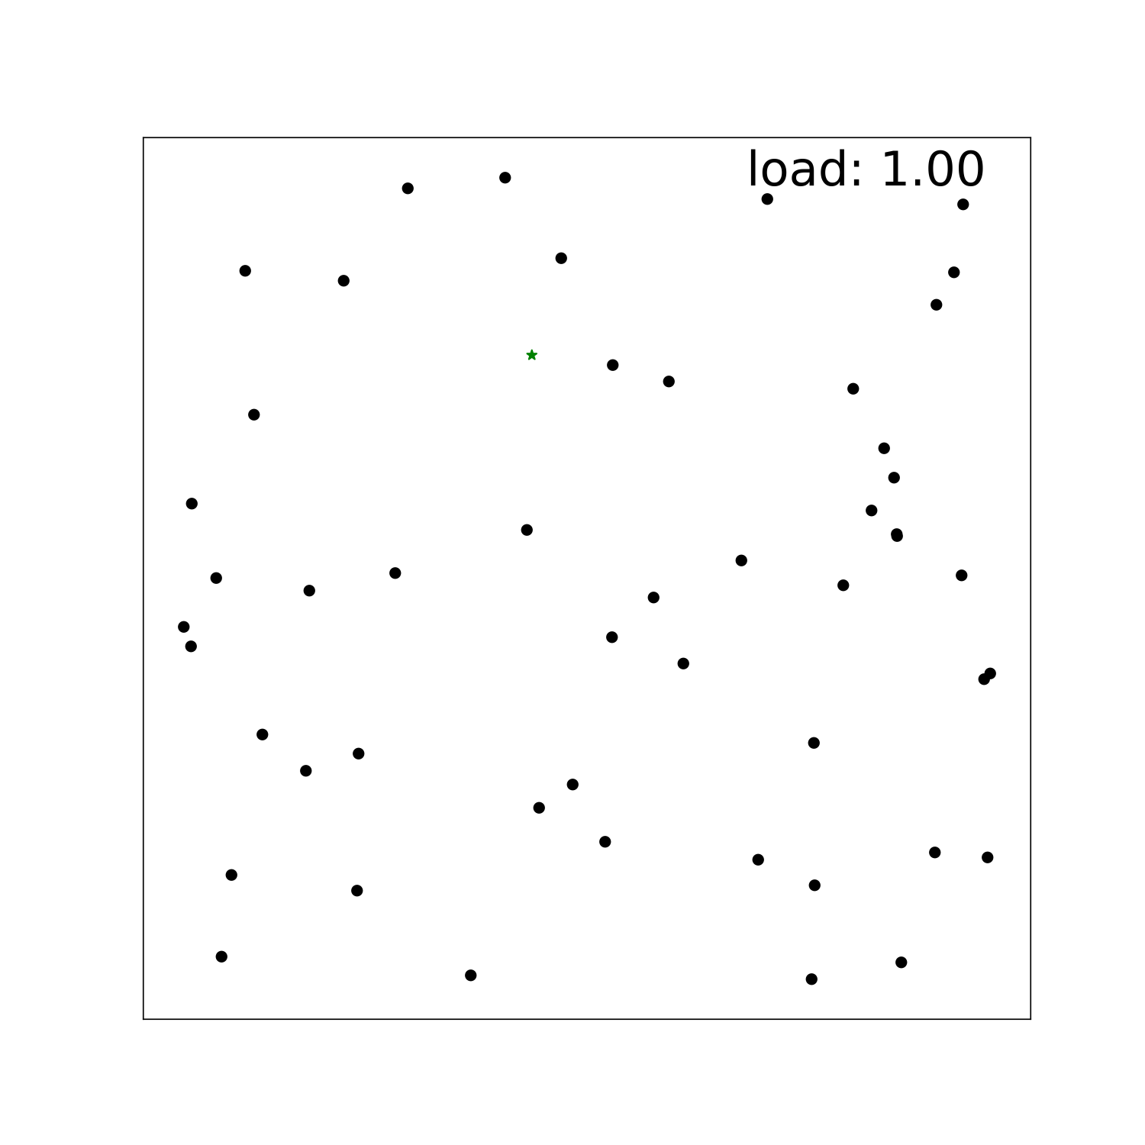
\includegraphics[width=\linewidth]{figures/50-0-am.png}
        \caption{initial}
        \label{fig:cvrp-50-initial}
    \end{subfigure}
    \begin{subfigure}[]{0.32\linewidth}
        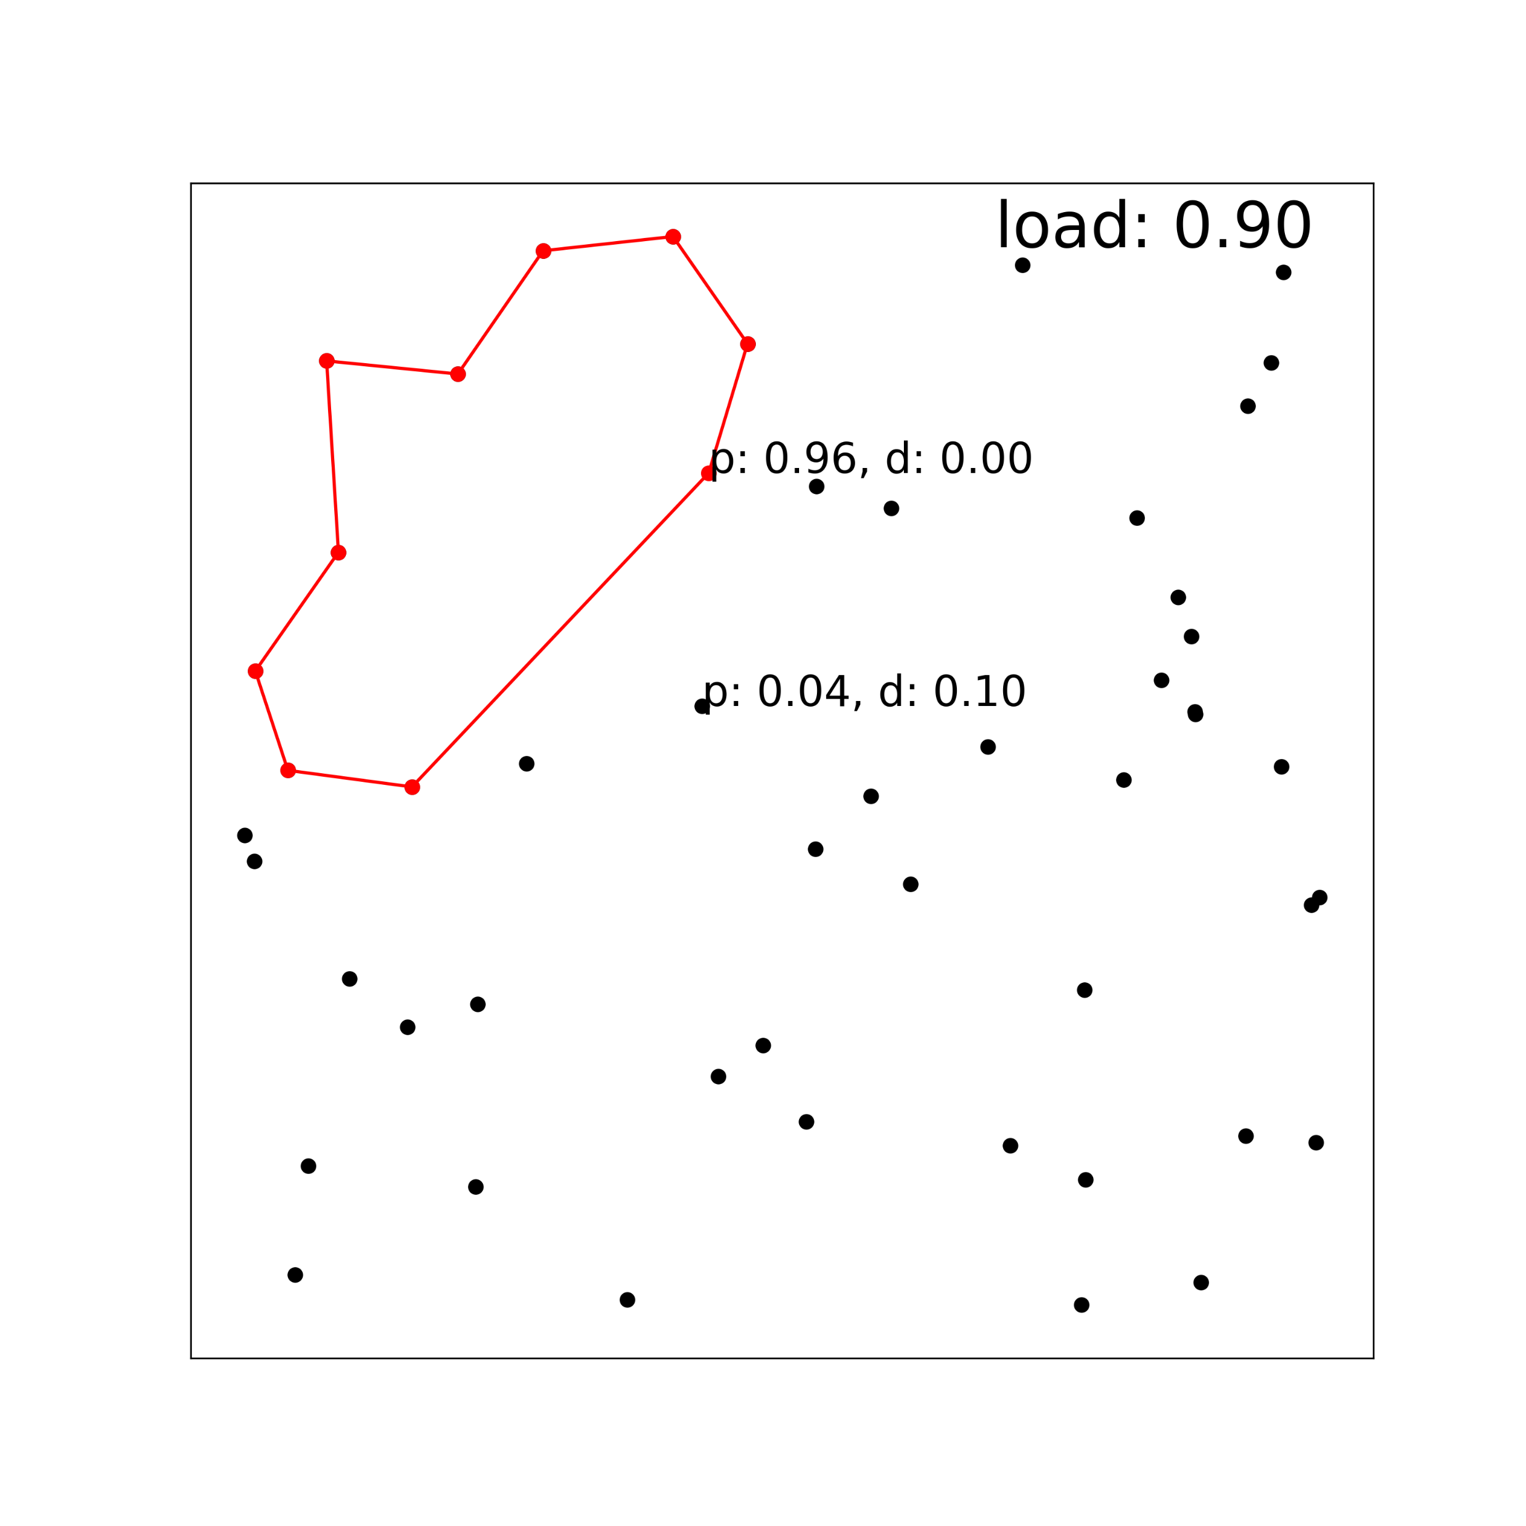
\includegraphics[width=\linewidth]{figures/50-11-am.png}
        \caption{first refill}
        \label{fig:cvrp-50-one_subroute}
    \end{subfigure}
    \begin{subfigure}[]{0.32\linewidth}
        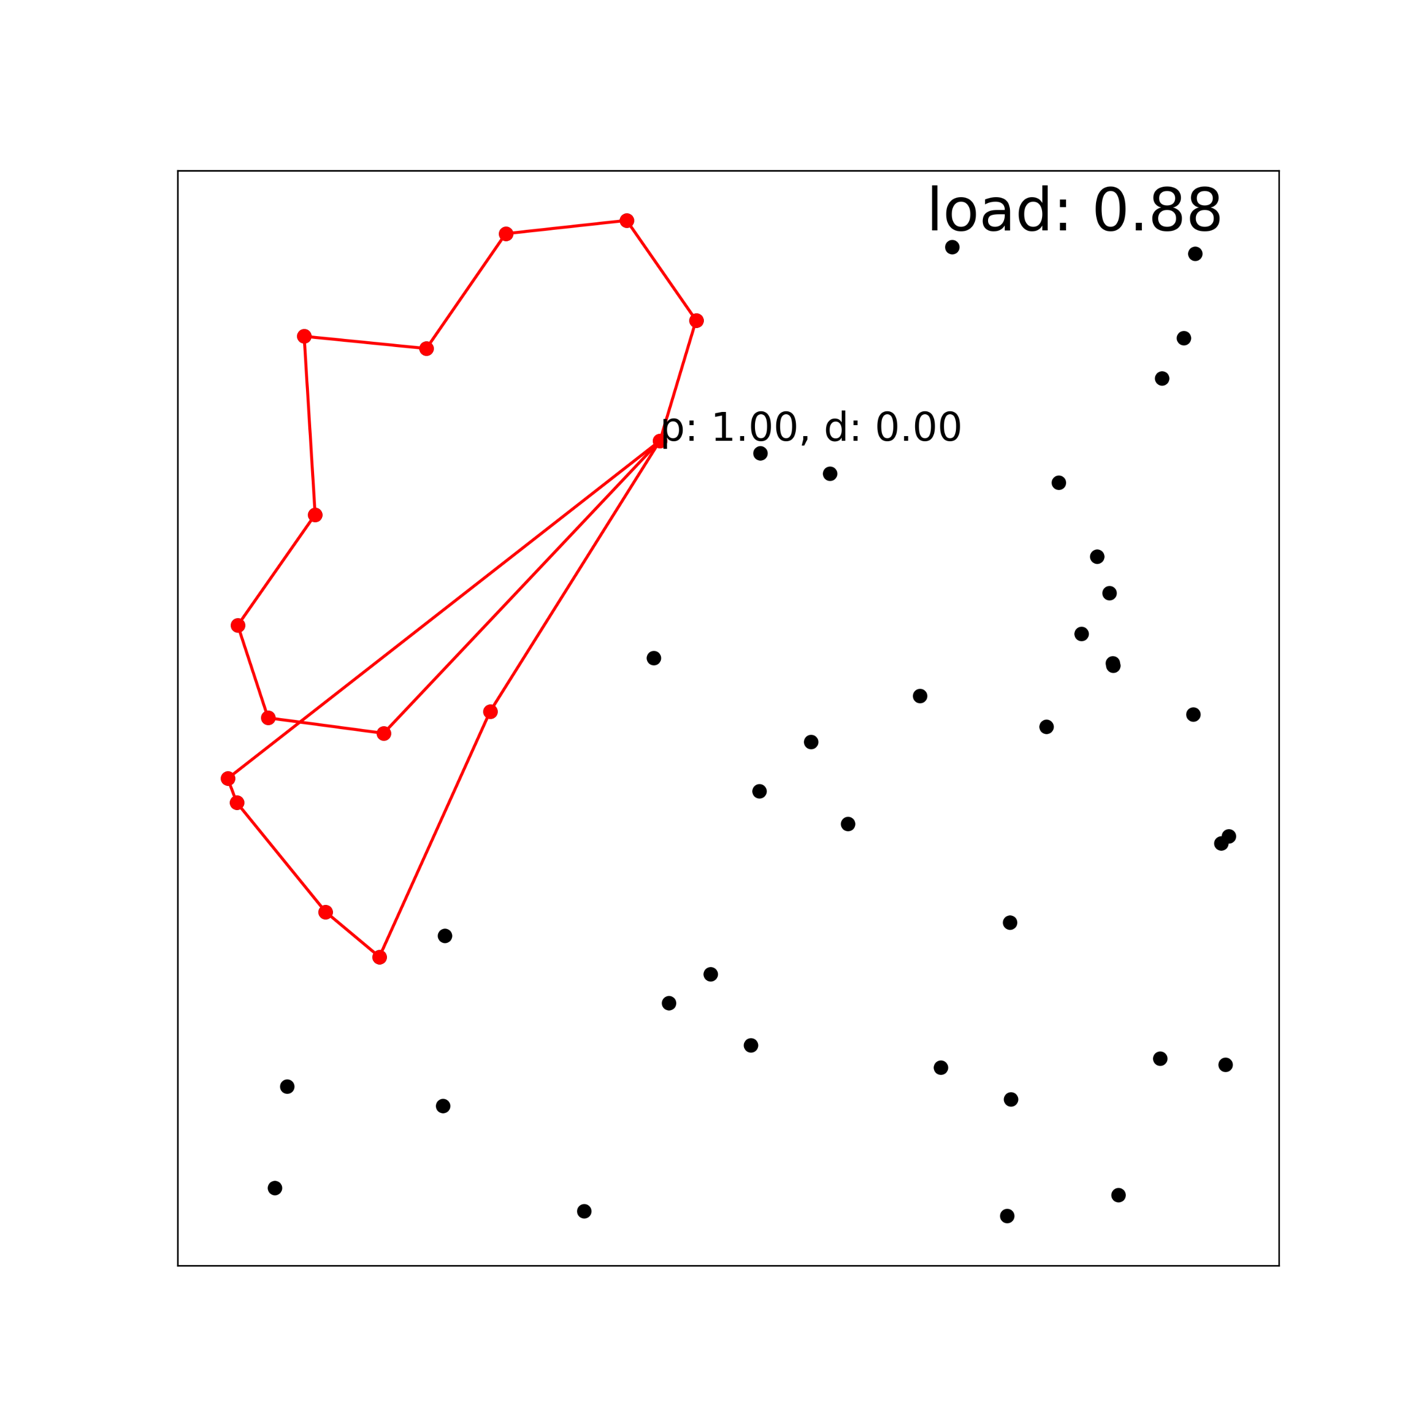
\includegraphics[width=\linewidth]{figures/50-17-am.png}
        \caption{second refill}
        \label{fig:cvrp-50-two_subroutes}
    \end{subfigure}
    \caption{Routing result in dynamic load settings}
    \label{fig:dynamic load setting figures}
\end{figure}

For example, as described in Figure \ref{fig:dynamic load setting figures}, we present a scenario where the vehicle refills with a smaller amount of load for a reason after its first subroute is created and solved with DRL. In the figure, dots represent customer nodes and red dots denote the nodes visited which are also connected by the red line. Figure \ref{fig:cvrp-50-initial} represents the initial setting with $Q^{max}=1$, Figure \ref{fig:cvrp-50-one_subroute} shows the situation after the vehicle and is refilled with a slightly different $Q^{max}=0.9$, and Figure \ref{fig:cvrp-50-two_subroutes} shows the routing result with $Q^{max}=0.9$. Usually, to handle these dynamics of the environment, a complicated mathematical formulation or expert engineering techniques are needed \cite{dynamicVRP}. However, with DRL, one can just adjust $Q^{max}$, which needs only one line to be changed in our implementation.


As a graph representation of the problem is common in the literature, we also represent the problem using a graph $G(V, E)$ where $V = \{0, 1, \cdots, n, n+1 \}$, meaning all the nodes in the problem: $0$ and $n+1$ are the \textit{same} depot node. The last node, $n+1$, is just an extra term for the ease of the formulation as the final depot of a tour. We define $\pi_t$ to be the node visited at time $t, t \ge 0$ with $\pi_0 = 0$ and a tour, $\boldsymbol{\pi}_{t_1,t_2}$, from time $t_1$ up to $t_2$ is defined as a sequence of visited nodes: for example, $\boldsymbol{\pi}_{0,T} = [\pi_0=0, \pi_1=2, \pi_2=7, ..., \pi_{T}=n+1]$, in which $T$ is the last time point in the tour. The terms route and tour are used interchangeably. Additionally, $E=\Set{(i,j)}{i, j \in V}$ means all the edges from all node combinations. Note that the demand of depot node $q_0$ is $0$, meaning $q_0=q_{n+1}=0$. We also introduce a binary decision variable $x_{ij}$ which is $1$ if there is a direct route from customer $i$ to $j$, and $0$ otherwise.
The distance of edge $(i,j)$ is denoted by $c_{ij}$.
The cost $C(\boldsymbol{\pi}_{0,t})$ is the cumulative distance calculated so far at $t$, given the sequence of visited nodes: $C(\boldsymbol{\pi}_{0,t}) = c_{\pi_0, \pi_1} + \cdots c_{\pi_{t-1}, \pi_{t}}$, and $C(\boldsymbol{\pi}_{0,0}) = 0$.
Lastly, on the route up to a visit of node $j\in V$, a continuous variable $y_j$ represents accumulated demands and is dependent on the decision variable $x_{ij}$: for instance, on tour $\boldsymbol{\pi}_{0,3}=[\pi_0, \pi_1, \pi_2, \pi_3$], $y_{\pi_3} = q_{\pi_0} + q_{\pi_1} + q_{\pi_2} + q_{\pi_3}$. We formulate the one-vehicle CVRP as follows:


  \begin{align}
    \min_{\forall x_{i,j}} & \sum\limits_{(i, j) \in E} c_{ij}x_{ij}\\
    \nonumber \text{subject to} & \\
    & \sum_{\substack{j=1,j \neq i  }}^{n+1} x_{i j}=1,  & i=1, \ldots, n, \\
    & \sum_{\substack{i=0, i \neq h }}^n x_{i h}-\sum_{\substack{j=1,j \neq h }}^{n+1} x_{h j}=0, & h=1, \ldots, n, \\
    & \sum_{j=1}^n x_{0 j} = 1, & \\
    & y_i+q_j x_{i j}-Q^{max}\left(1-x_{i j}\right) \leq y_j , & i, j=0, \ldots, n+1, \\
    & q_i \leq y_i \leq Q^{max}, & i=0, \ldots, n+1, \\
    & x_{i j} \in\{0,1\}, & i, j=0, \ldots, n+1 .
  \end{align}

%${\color{red}XX: double-check $y_0$ to be consistent with the underneath.}
We briefly explain a list of equations as follows:
equation (1) is the objective of the problem, the minimization of the distance traveled by the vehicle; equation (2) is a constraint to regularize all customers being visited only once; equation (3) controls the correct flow of a tour, the visit sequence, by ensuring the number of times a vehicle enters a node is equal to the number of times it leaves the node; equation (4) imposes that only one vehicle leaves the depot; equations (5) and (6) jointly express the condition of vehicle capacity. Note that variants for the constraints are possible, and the main reference to the above formulation is \citet{CVRPLP}. We also notice that the finding of solution $x_{i,j}$ is equivalent to the construction of tour ${\boldsymbol{\pi}_{0,T}}$: for example, $\pi_1=2, \pi_2=7$ represent $x_{2,7}=1$.
Noticeably in the formulation, the finding of $x_{ij}$ leads to the construction of $y_i$.
To migrate this formulation into TSP, one only needs to remove constraints regarding the capacity of a vehicle and the demands of customers, so that only decision variable $x_{ij}$ remains.

\section{Proposed Network Model, AlphaRouter}

\begin{figure}
    \centering
    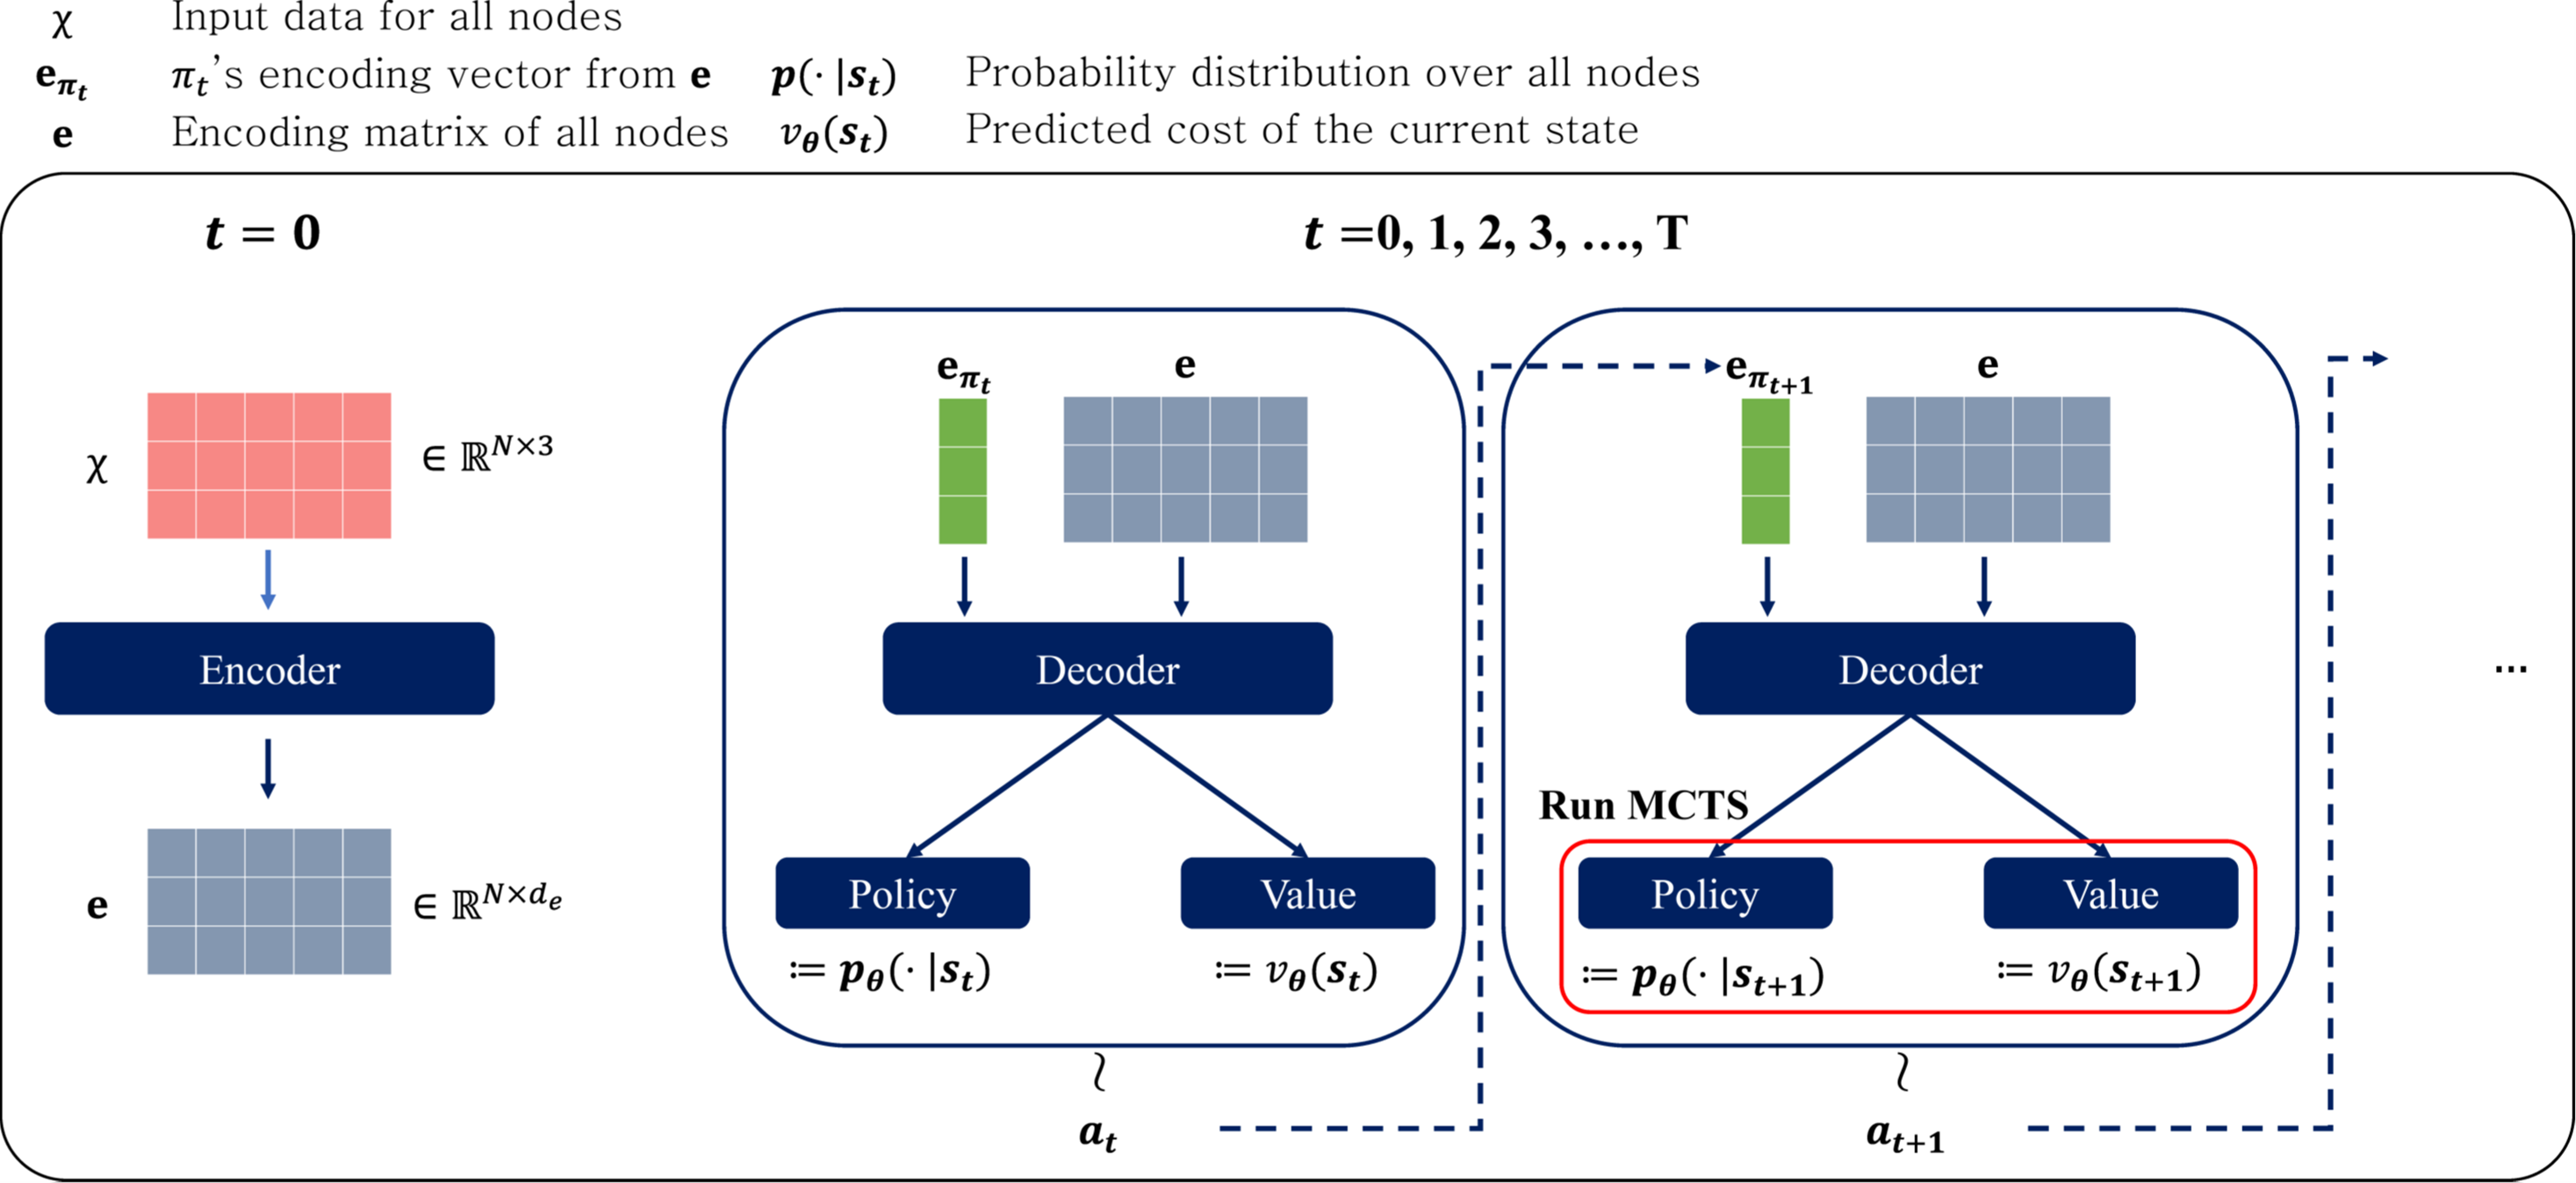
\includegraphics[width=0.98\linewidth]{figures/overall.png}
    \caption{Overall process of routing using our proposed neural networks is shown. It auto-regressively selects the next node. The encoder is executed once per episode, and the decoder is executed at every timestep $t$.}
    \label{fig:nn-overall}
\end{figure}


In this section, we present our approach, named AlphaRouter, to solving the routing problem using both reinforcement learning and MCTS frameworks.
We revise the above routing problem by adding the possibility of refilling the vehicle to reflect realistic situations. We notice that the above routing problem is unable to include the refilling action.
We begin by defining the components to bring the environment into our RL problem, followed by neural network models of policy and value. We then outline our idea and implementation to adapt MCTS to the routing problem. Our overall process consists of two stages: training the neural network using reinforcement learning and combining the pre-trained network with the modified MCTS strategy to search for a better solution, meaning tour ${\boldsymbol{\pi}_{0,T}}$ or $x_{i,j}$ in the CVRP formulation.
%When applying the MCTS to all selections, it is time-consuming.
Due to computational demands associated with the application of MCTS, we adopt a selective application of our MCTS when ambiguity arises in choosing the next customer node that is proposed by the output distribution of the policy network, in which the output distribution means the distribution of possible next nodes. This selective application enhances computational efficiency while maintaining the effectiveness of the MCTS strategy.

\subsection{Reinforcement Learning Formulation}
% need to add a figure that shows the overall sequence of the algorithm. i.e., from input x to intermediate decoder output and then policy, value. Explaining the denoted notations should be more practical.

The input is denoted by $\mathbf{x}_i \in \mathbb{R}^2$ which represents a set of coordinates for customer $i$. The demand of node can be included in the vector if the problem is a type of CVRP: i.e., the input for CVRP is then $[\mathbf{x}_i; q_i] \in \mathbb{R}^3$, where semicolon $;$ represents a concatenation operation. Also, with $n$ customers, the total number of nodes is $N=n$ for TSP, and $N=n+1$ for CVRP as one depot node exists. Thus, the input matrix is denoted as $\mathbf{\chi} = \mathbf{x} \in \mathbb{R}^{N\times 2}$ for TSP problems, and $\mathbf{\chi} = [ \mathbf{x}_i; q_i] \in \mathbb{R}^{N \times 3}$ for CVRP.

%$\HWG{XX: In this subsection, it needs to mention an episode, the $t$(?) step of node selection -- the meaning of Figure 1. }
%\subsection{Formulation of Our Neural Network for Reinforcement Learning}

To bring the problem into a reinforcement learning framework, we define the state, action, and cost (converted to reward). In our work, the observation state at timepoint $t$, denoted by $s_t$, is a collection of the node data $\chi$, containing coordinates and demands, the currently positioned node $\pi_t$, a set of available nodes to visit, denoted by $V_t$, and a masking vector for unavailable nodes $m_t \in \mathbf{R}^N$ of which $p^{th}$ element in the vector is filled with $0$ if $p \in V_t$ and $-\infty$ if $p \notin V_t$: $s_t = (\chi, \pi_t, V_t, m_t)$.
Though masking vector $m_t$ stems from available-node set $V_t$ in our formulation, we intentionally add both $m_t$ and $V_t$ to the state $s_t$ so that the masking vector may be adjusted and redefined reflecting domain requirements just as several masking techniques are possible in Transformer \cite{masked_attention, vaswaniAttentionAllYou2017, masked_attention2}  .

We omit $t$ for $\chi$ as the node data is invariant over time in this problem: for all time points, $\chi$ stays unchanged. However, one could make node data $\chi$ varying in time depending on the domain requirement, and the proposed network model is able to handle time-varying $\chi$.
For CVRP, the current vehicle's load, denoted by $\mbox{load}_t = Q^{max} - y_{\pi_t}$, is also added to $s_t$: $s_t = (\chi, \pi_t,  V_t, m_t, \mbox{load}_t)$.
The node set $V_t \subset V$ holds nodes, not visited yet, that are able to fulfill the demands considering $\mbox{load}_t$.

The action, denoted as $a_t$, is to choose the next customer node and move to it. The action in an episode, a sequence of possible states, is chosen by our policy neural network, as shown in Figure \ref{fig:nn-overall}, which outputs a probability distribution over all the nodes given the state at $t$, $s_t$. We use $p_\theta(.|s_t)$ to describe the policy network output at time $t$ during the episode rollout. In the training phase, the action is sampled from action distribution $p_\theta(.|s_{t})$, $a_{t} \sim p_\theta(.|s_{t})$, as the next node to visit, meaning $\pi_{t+1}=a_t, t \ge 0$, with $\pi_0 = 0$. The sampling operation aims to give the vehicle (or agent) a chance to explore a better solution space in our training phase. In the inference phase, however, we choose the action with the maximum probability, meaning $\hat{a}_{t} = \argmax_{i \in V_t}{p_\theta(i|s_t)}$ if unvisited nodes exist, and $\hat{a}_{t} = n+1$ otherwise.

A value network is designed to predict an overall cost (or distance), in the episode at state $s_t$. This is later used in updating the MCTS tree's statistics. We will describe in detail how other components work in the next subsection.
Specifically, an episode, $\tau$, is a rollout process in which state and action are interleaved over $t=0,1, \cdots, T$ until the terminal state $s_T$ is reached: $\tau=(s_0,  a_0, C(\boldsymbol{\pi}_{0,0}), \cdots, s_T,  a_T, C(\boldsymbol{\pi}_{0,T}))$. In this problem, the terminal state is the state in which all customers are visited and the vehicle has returned to the depot if it is CVRP. Because of possibly multiple refillings of the vehicle, the last time point $T$ can be different in episodes of CVRP problems. For example, even when the problems have the same size (for example, $n=50$), the optimal solution path can be different due to different customer locations and demands. Upon reaching the terminal state, no more transitions are made, and the overall distance, $C(\boldsymbol{\pi}_{0,T})$, is calculated.

% \HWG{XX: Need to relate it to Figure 1. It needs to mention the value network. It needs to mention $e_0$ and $e_1$.}

\subsection{Architecture of the Proposed Network Model}

The neural network architecture of our policy network for calculating the probability distribution $p_\theta(\cdot|s_t)$ is similar to the one used in previous studies \cite{kool2018attention, kwonPOMOPolicyOptimization2021}. However, to solve the routing problem, we modified the decoder part, relying on the transformer \cite{vaswaniAttentionAllYou2017}. We aim to extract meaningful, possibly highly time-dependent and complex, features that are specific to the current state while maintaining the whole node structure.
We make the two networks share the same embedding vector, transformed by the current input, $s_t$ at time $t$. The design of the shared input transformation is a deep-layered network, consisting of an encoder and decoder, to fully take advantage of both the whole node structure and the current node.
The structure of the two networks with the shared feature transformation is reminiscent of the architecture from the AlphaGo series \cite{silverMasteringGameGo2016, silverMasteringGameGo2017} and the previously related works \cite{kool2018attention, kwonPOMOPolicyOptimization2021}. In essence, the input $s_t$ produces the estimated probability of possible next actions via the policy network, $p_\theta(\cdot |s_t)$, and the predicted cost via the value network, $v_\theta(s_t)$. For simplicity, we denote all learnable parameters as $\theta$, actually consisting of parameters from the shared transformation, those from the policy network, and those from the value network.

In detail, we explain the proposed network, dividing it into three parts: encoder in the feature transformation, decoder in the feature transformation, and policy \& value. The objective of the encoder is to capture the inter-relationship between nodes. The encoder takes only the node data input $\chi$ from the $s_t$, passing it to a linear layer to align with a new dimensionality, $d_e$, via the multi-head attention layers, expressed by $MHA(\boldsymbol{Q}, \boldsymbol{K}, \boldsymbol{V})$ with input tensors of query $\boldsymbol{Q}$, key $\boldsymbol{K}$, and value $\boldsymbol{V}$. The output of the multi-head attention is an encoding matrix, denoted by $\mathbf{e} \in \mathbb{R}^{N \times d_e}$. Each row vector represents the $i^{th}$ node in the encoding matrix, denoted by $\mathbf{e}_i \in \mathbb{R}^{d_e}$. So, the currently positioned node at time $t$'s encoding is $\mathbf{e}_{\pi_t}$, the embedding vector reflecting the complex and interweaved relationship with the other nodes. In summary, the encoder process is self-attention to the input node data expressed as $\mathbf{e} = MHA(Linear(\chi), Linear(\chi), Linear(\chi))$. This is repeated over several layers in the model. Relying on the idea of hidden states and current inputs in recurrent networks, we execute encoder process once \textit{per episode}, thereby reducing the computational burden, and use the current-node embedding and the current loading $\mbox{load}_t$ as inputs to the decoder in a sequential manner. We provide a detailed explanation later in this section.

The decoder is responsible for revealing the diluted relationships in the encoding matrix $\mathbf{e}$ with additional information if it is given. Specifically, the decoder captures the relationships between the current node $\chi$ and the others. For example, let us assume that the vehicle is currently on node $i$ and the current node's embedding is $\mathbf{e}_i$. Notice that we ignore time $t$ in the encoding matrix since it does not change in an episode as the output of the encoder is reused over the episode once it has been executed. %\HWG{XX: is it correctly written?}
By using this $\mathbf{e}_i$ as the query and the whole encoding matrix $\mathbf{e}$ as key and value, the decoder can reveal the relationships between the current node and the others. When passing the query, key, and value, we apply linear transformations to each of them. One should note that TSP and CVRP have different inputs for the query. In CVRP, the current load, $\mbox{load}_t \in s_t$ is appended to the query input while TSP is not. While there are several layers for the encoder, we only use one layer of MHA for the decoder. A summarization of the decoder is as follows:



\begin{align}
    & \mathbf{d} = MHA(\boldsymbol{Q}, \boldsymbol{K}, \boldsymbol{V}) \in \mathbb{R}^{d_e}, \\
    & \boldsymbol{Q} =
    \begin{cases}
         \mbox{Linear}(\mathbf{e}_{\pi_t}) & \text{for TSP}, \\
         \mbox{Linear}([\mathbf{e}_{\pi_t}; load_t]) & \text{for CVRP},
    \end{cases} \\
    & \boldsymbol{K} = \mbox{Linear}(\mathbf{e}),~~ \boldsymbol{V} = \mbox{Linear}(\mathbf{e}).
\end{align}

\begin{figure}
    \begin{center}
        \begin{subfigure}[b]{0.45\linewidth}
        \centering
         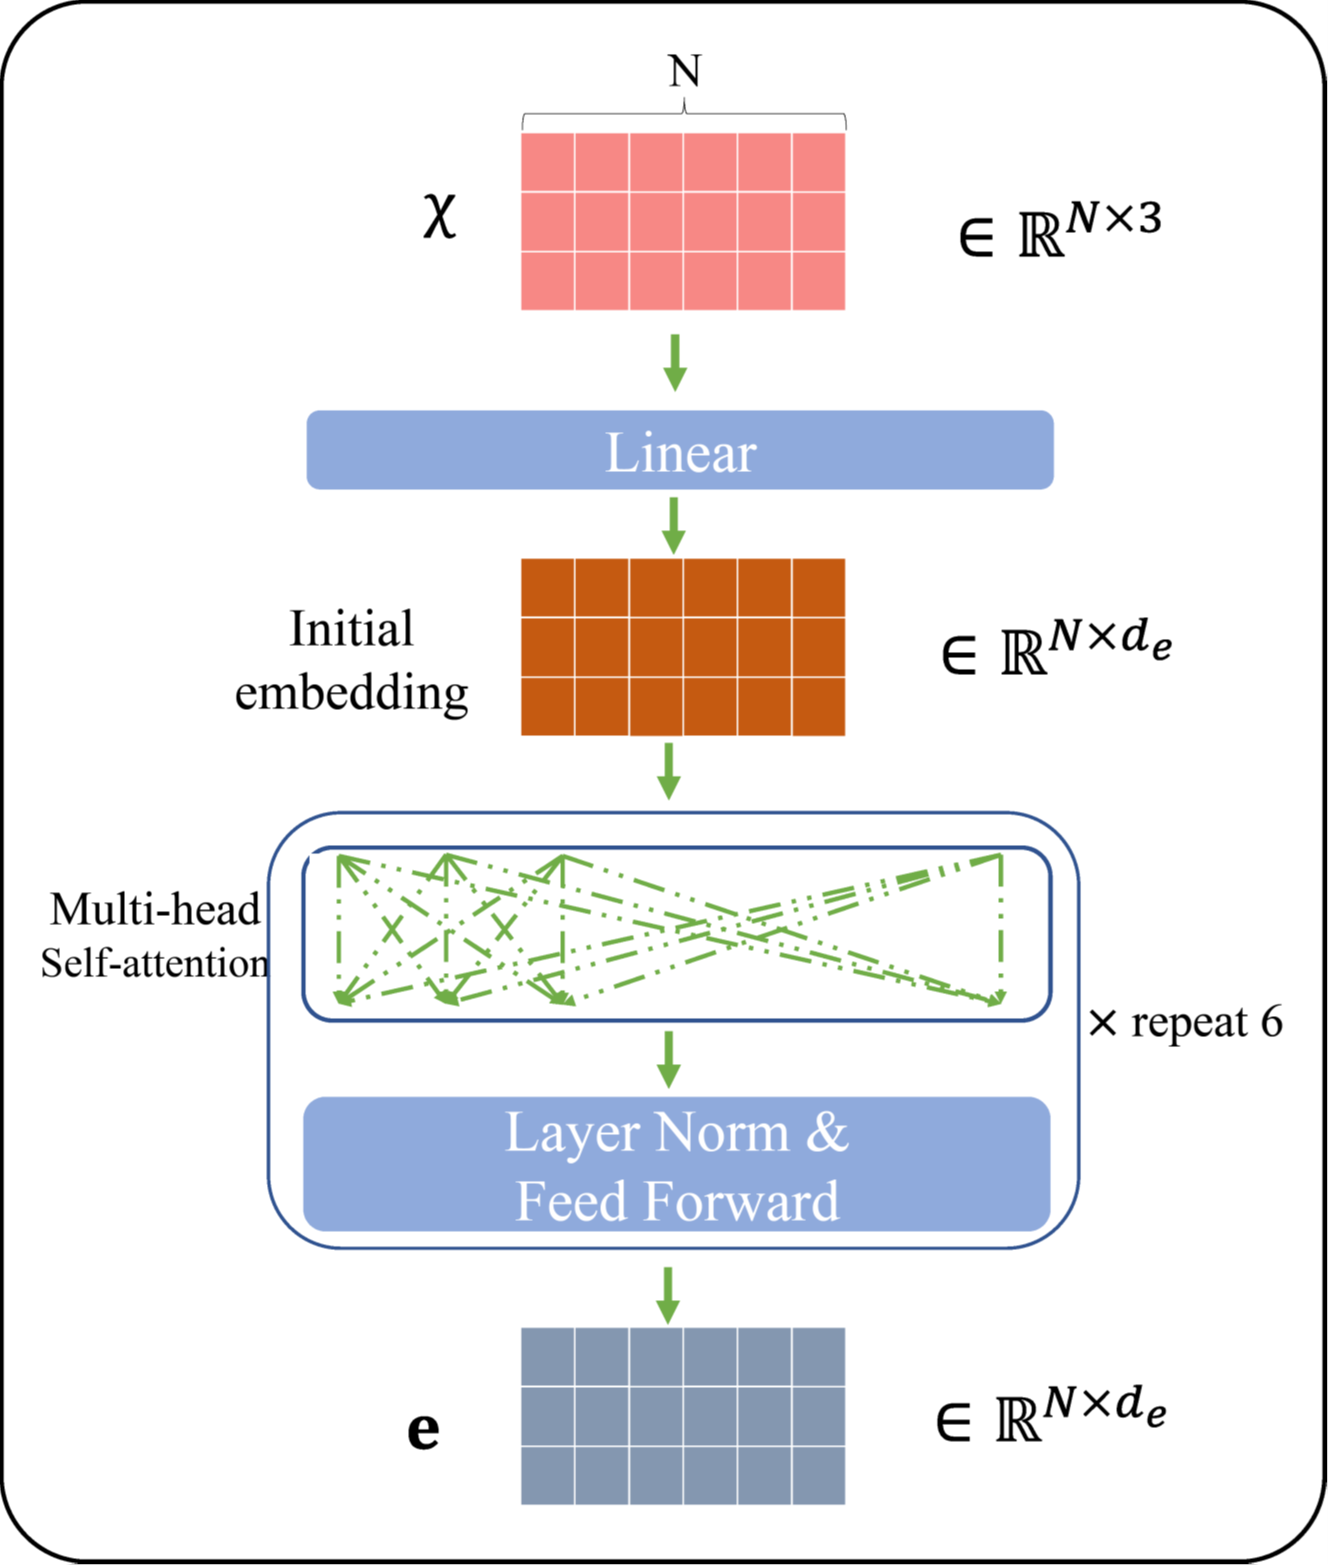
\includegraphics[width=\linewidth]{figures/encoder.png}
         \caption{encoder}
         \label{fig:nn-encoder}
        \end{subfigure}
        \hfill
        \begin{subfigure}[b]{0.45\linewidth}
            \centering
             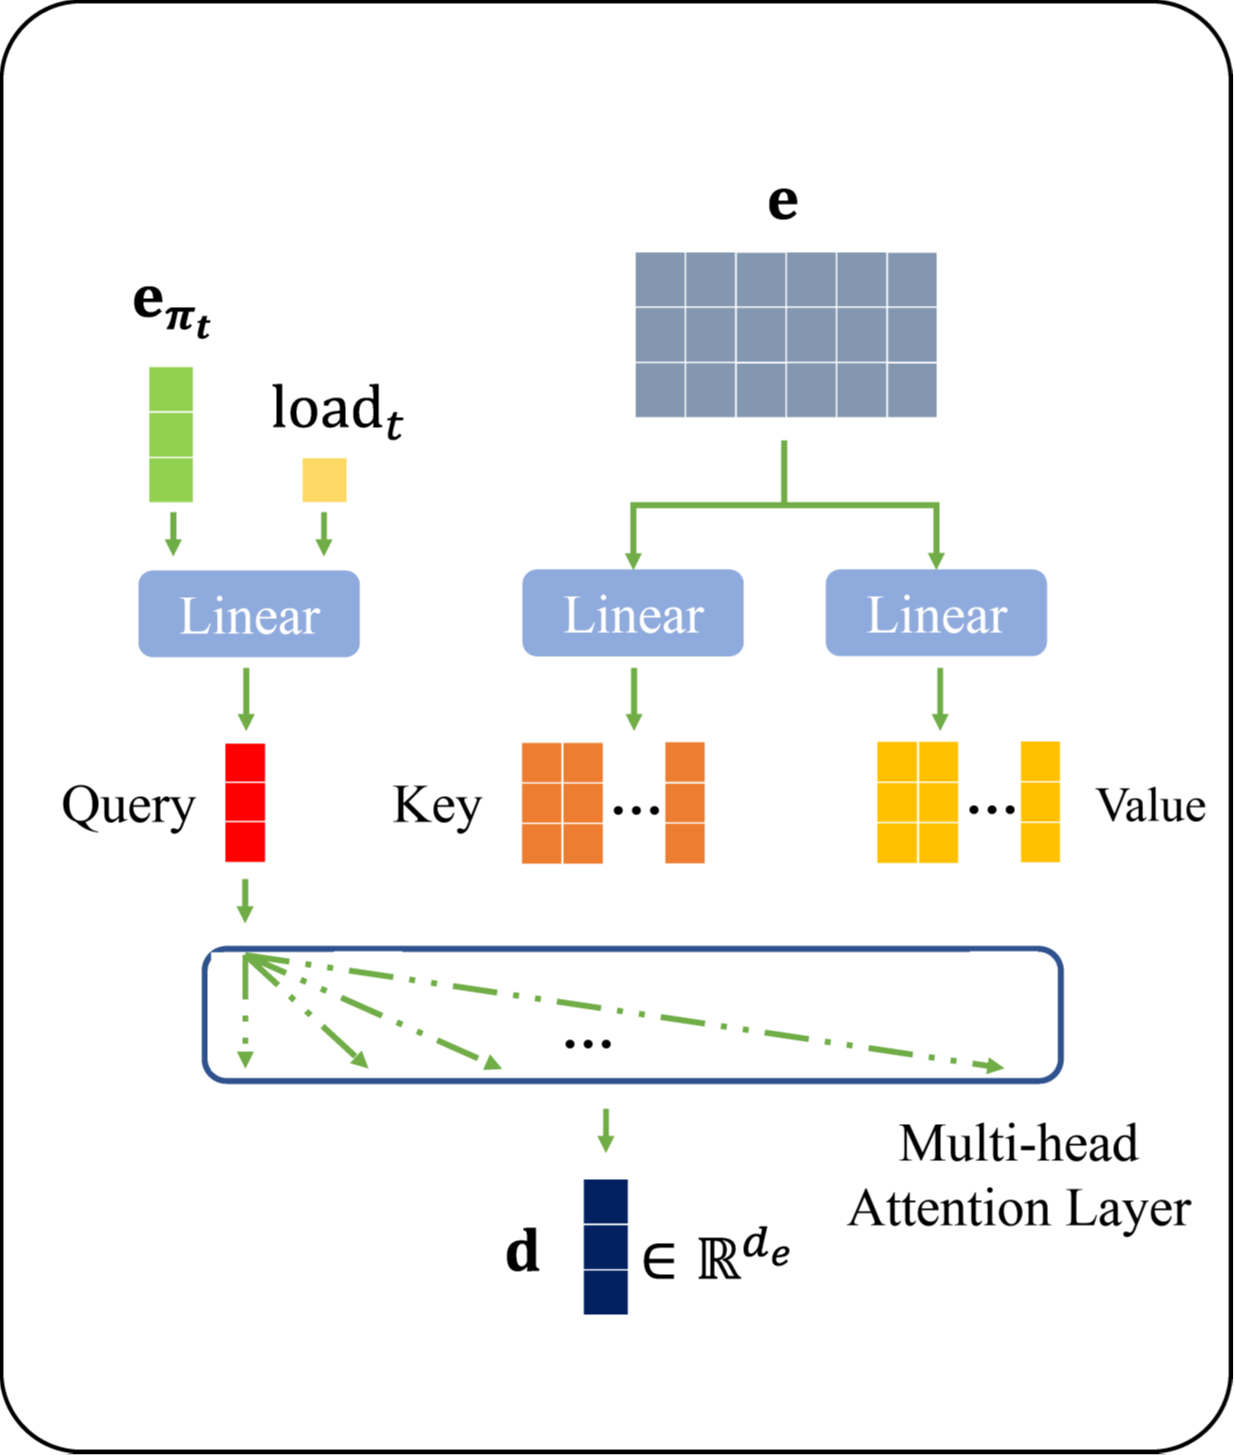
\includegraphics[width=\linewidth]{figures/decoder.png}
             \caption{decoder}
             \label{fig:nn-decoder}
        \end{subfigure}
    \end{center}

    \centering
    \begin{subfigure}[b]{0.95\linewidth}
         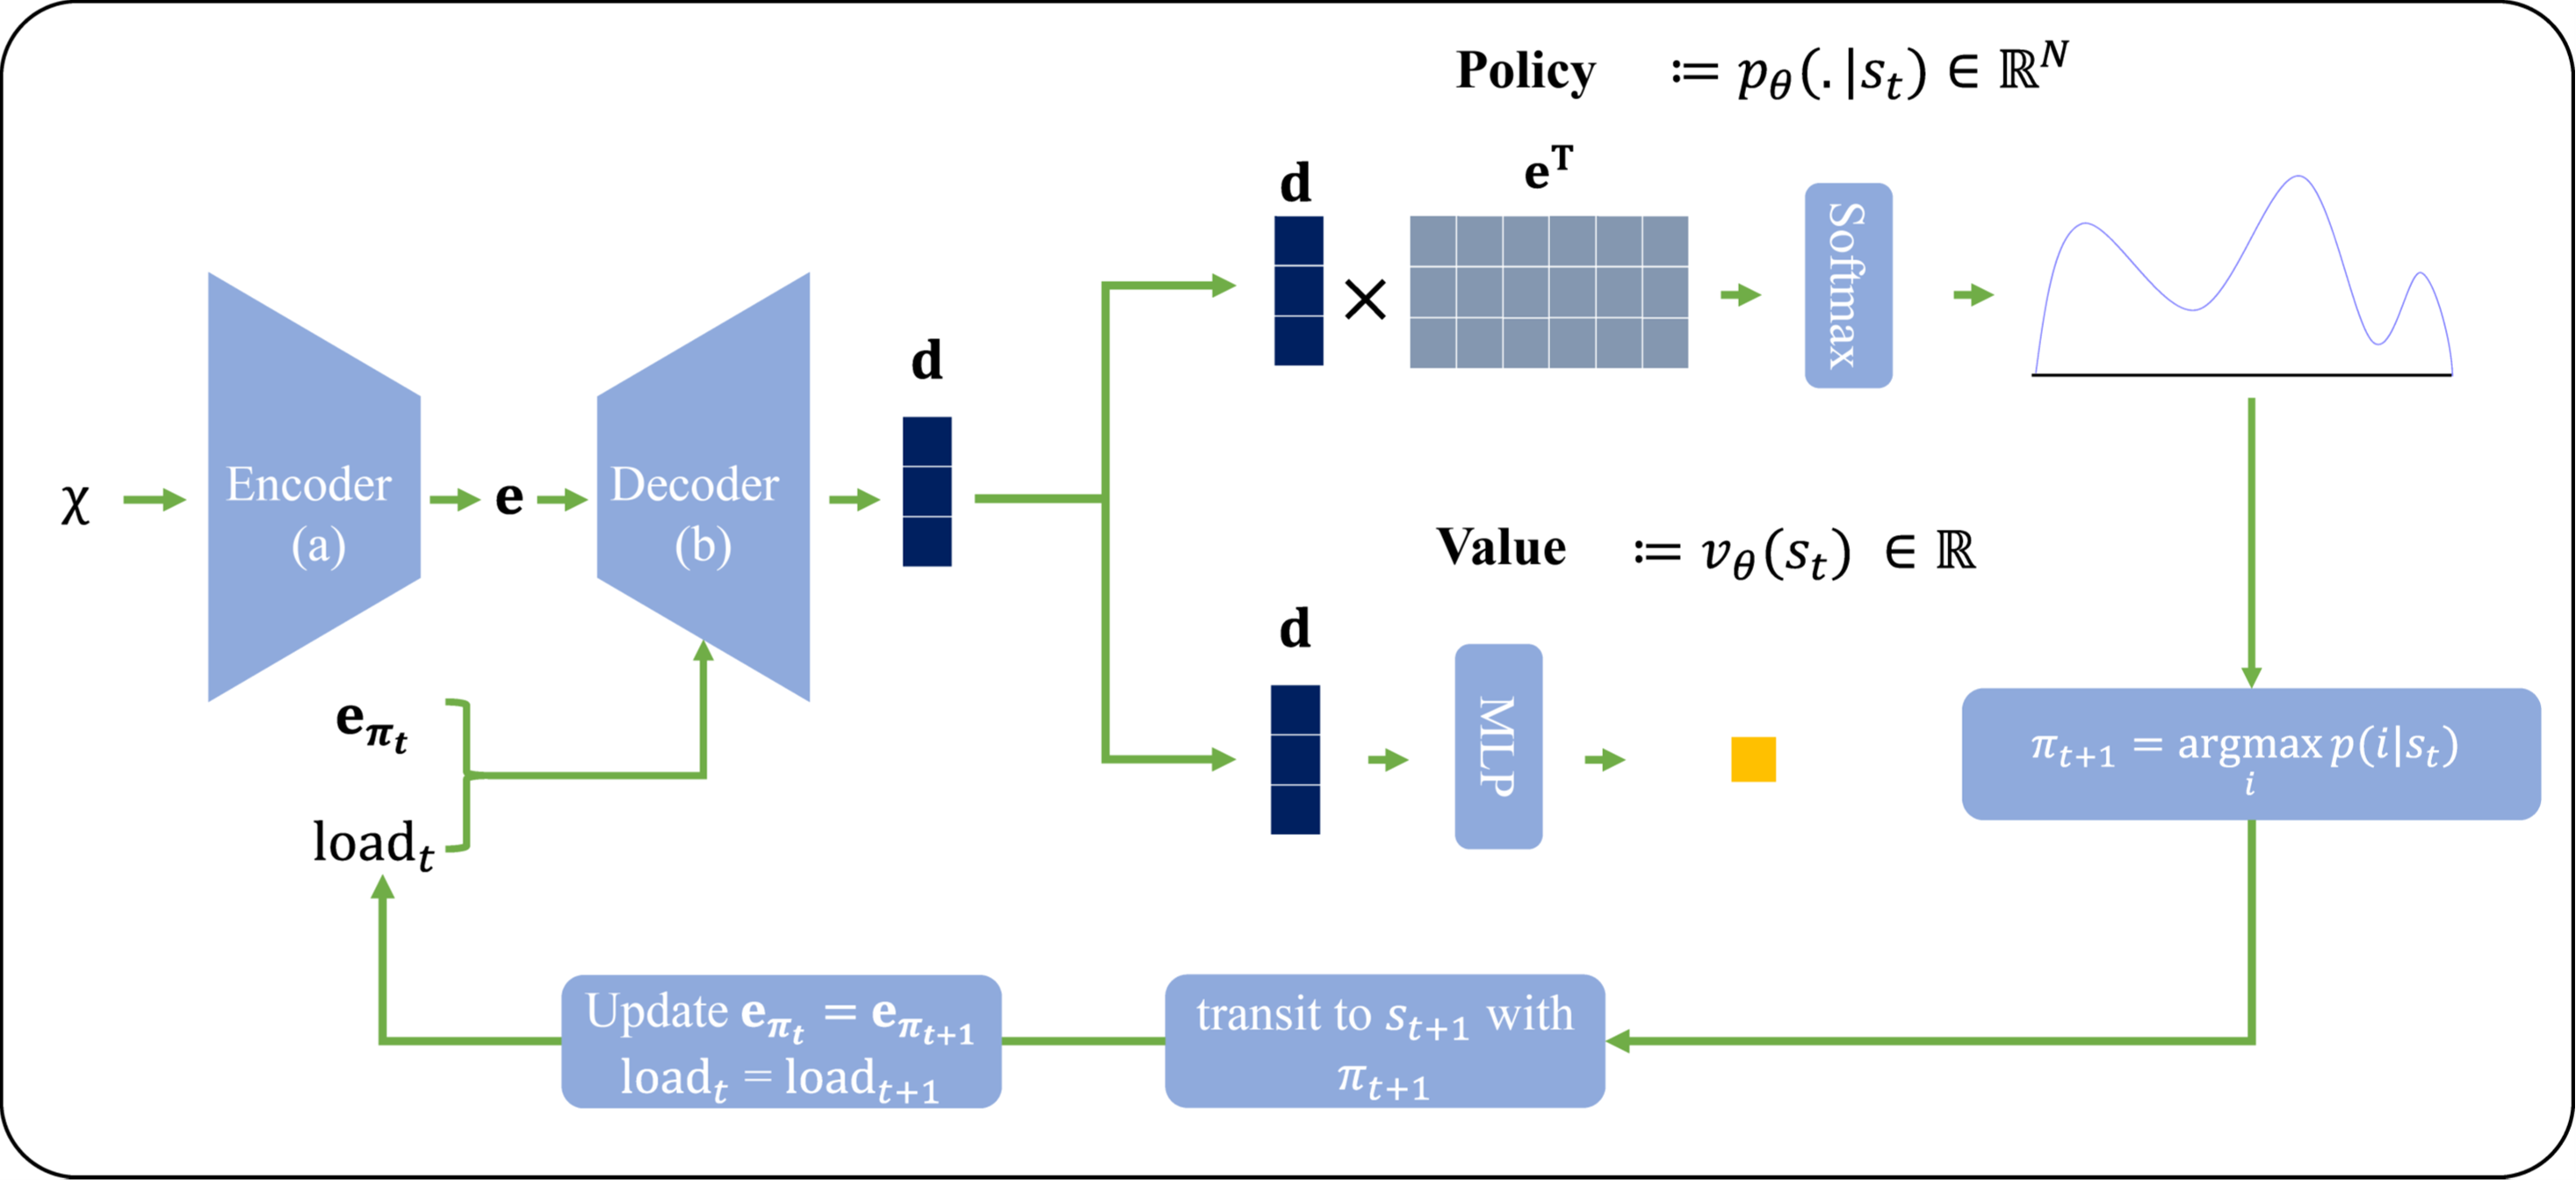
\includegraphics[width=\linewidth]{figures/policy and value - integrated.png}
         \caption{policy \& value}
         \label{fig:nn-policy_and_value}
    \end{subfigure}
    \caption{Components of the neural network}
    \label{fig:neural net components}
\end{figure}

The policy layer and value layer are responsible for calculating the final policy $p_{\theta}(\cdot | s_t)$, a probability distribution on all nodes given $s_t$, and the predicted distance $v_{\theta}(s_t)$ output respectively. We compute $p_{\theta}(\cdot | s_t)$ as follows with a given hyper-parameter $C$ that regulates the clipping:

%\begin{align}
%    masked \_ logit = tanh(\mathbf{d}\mathbf{e}^T  / \sqrt{d_e})C + m_t, \\
%    p_{\theta}(\cdot | s_t) = Softmax(masked \_logit).
%\end{align}
\begin{align}
    p_{\theta}(\cdot | s_t) = \mbox{softmax}(\mbox{tanh}(\mathbf{d}\mathbf{e}^T  / \sqrt{d_e})C + m_t).
\end{align}
To compute $p_{\theta}(\cdot | s_t)$, we multiply the decoder output $\mathbf{d}$ by the transposed encoding matrix $\mathbf{e}^T$ and divide it by $\sqrt{d_e}$. The output goes through the tanh function, and we add the mask for the nodes unavailable $m_t$ to it. Finally, we apply a softmax operator to this result.


For $v_{\theta}(s_t)$, we pass the same decoder output $\mathbf{d}$ to two linear layers of which the shape is similar to the usual feed-forward block in the transformer: $v_{\theta}(s_t) = \mbox{Linear}(\sigma(\mbox{Linear}(\mathbf{d})))$, in which $\sigma(\cdot)$ is an activation function such as ReLU and SwiGLU \cite{agarap2018ReLU, shazeer2020swiglu}. A diagram for each neural network design is illustrated in Figure \ref{fig:neural net components}.

For training the model for an episode, the encoding process is only required once as the input of the encoder (the coordinates of nodes) is fixed along the rollout steps. The decoder, on the other hand, takes the inputs that change over time, i.e., the current node and current load. Thus, on the first execution of the model, we execute both the encoder and the decoder. After the first execution, we execute only the decoder and policy and value parts, saving considerable computations. Noticeably the encoder and decoder share the same parameters while the policy and value networks do not. Figure \ref{fig:nn-overall} explains the overall process.

Additionally, we intentionally exclude residuals in the encoder layers as we have observed that, unlike the original transformer and its variants, residual connections greatly harm the performance of the model. %We point out the performance difference in section 5.2 of the ablation study.
Another variation we have added to the previous is the activation functions. Recent studies on large language models (LLMs) exploited different activation functions for their work. We took this into account and tested SwiGLU activation, just as Google's PaLM did in \cite{chowdhery2022palm}. We report the results in later sections.

\subsection{Training the Neural Network}

To train the policy network $\theta$, we use the well-known policy gradient algorithm, `reinformce with the baseline'\cite{williamsREINFORCE}. This algorithm deals with high variance problems prevalent in policy gradient methods by subtracting a specially calculated value, called the baseline. This algorithm collects data during an episode and updates the parameters after each episode ends.
%For the sake of notation, we define $S$ as a problem set of all possible cases, $s_t \in S$,
%$\mathbf{\chi} = [ \mathbf{x}_i; q_i]$ containing node data, coordinates and demands.
%${\color{red}XX: is $s$ different from $s_t$, a state at time $t$?}
%and $L(\boldsymbol{\pi})$ to be the distance traveled by the vehicle following the sequence $\boldsymbol{\pi}$, equal to $c_T$.
For $C(\boldsymbol{\pi}_{0,T})$, the distance traveled by the vehicle following the sequence $\boldsymbol{\pi}_{0,T}$,
the policy network aims to learn a stochastic policy that outputs a visit sequence with a small distance over all problem instances. The gradient of the objective function for the policy network is formulated as follows:

\begin{align}\label{eqn:gradient-of-policy-objective1}
        & \nabla J_\theta(\boldsymbol{\pi}) \varpropto \mathbb{E}_{\boldsymbol{\pi}
 \sim p_\theta(\cdot |\boldsymbol{s})}[(C(\boldsymbol{\pi}_{0,T}) - b(\boldsymbol{s}))\nabla \log p_\theta(\boldsymbol{\pi}|\boldsymbol{s})],
 \end{align}
 \begin{align*}
        & \text{where}~ p_\theta(\boldsymbol{\pi} | \boldsymbol{s}) = p_\theta(\pi_0 | s_0) \prod_{k=1}^{T-1}p_\theta(\pi_k | s_k, \pi_{k-1})
\end{align*}

in which $b(\boldsymbol{s})$ is a deterministic greedy rollout from the best policy trained so far as a baseline to reduce the variance of the original formulation \cite{kool2018attention}. In detail, after training model parameter $\theta$ for an epoch, we evaluated it with a validation problem set, setting $b(\boldsymbol{s})$ as the evaluated cost in the validation. One can think of this procedure as the training-validation mechanism in general machine learning.
%{\color{red}XX: in another roll-out, what is $s_0$? no need?}
The mere use of a baseline incurs additional computational costs arising from rollouts of several episodes, being an expensive procedure.
To alleviate this burden, we introduced a value network, $b(\boldsymbol{s})=v_\theta(\boldsymbol{s})$, instead of the greedy rollout baseline.

The value network's objective is to learn the expected cost at the end of the episode from \textit{any state} during the episode rollout. We keep track of the value network's output throughout a rollout and train the network with the loss function
    \begin{align}\label{eqn:value_objective}
            L_v \varpropto \sum_{t=0}^{t=T}(C(\boldsymbol{\pi}_{0,T}) - v_\theta(s_t))^2
    \end{align}

As in the POMO approach\cite{kwonPOMOPolicyOptimization2021}
%claimed that the mean of costs over all batches is better than the deterministic greedy rollout baseline ,
we tested a baseline using the average cost over a batch of episodes in addition to a baseline using value network $v_\theta(s_t)$. For instance, we calculate the baseline as the mean of all $64$ episodes as a batch size, representing the number of concurrent episode runs. This value network is also used in the MCTS process described in the next section. Since our model shares the parameters in the encoder and decoder between the policy network and the value network, an update in the value network affects the parameters in the policy network with the gradient of the final loss as follows:
%so that the gradient of the value loss flows into other parts of the model too {\color{red} XX: what is the meaning of $\sum_{t=0}^{t=T}(L(\pi) - v_\theta(s_t))^2$?}
%The gradient of the final loss is as follows:
    \begin{align}\label{total loss}
        \nabla \mathcal{L} \varpropto \nabla J_\theta(\boldsymbol{\pi}) + \nabla L_v.
    \end{align}

%----------------------------------------------------------------------------------------------------------------------------------------------------------------------------------------------
\subsection{Proposed MCTS for the Routing}

The main idea of MCTS is to improve the solutions, good in general, of trained policy and value networks to be problem-specific by investigating possible actions.
In essence, without MCTS, we make a transition from $s_t$ to $s_{t+1}$ by taking action $a_t$, which is the output from the policy network \textit{only}. However, in our proposed MCTS as described in Figure \ref{fig:nn-overall}, we select the next node by considering costs, which is the output of the value network, in addition to the prior probabilities from the policy network. In addition, we selectively apply the MCTS at time $t$ when the highest probability from the current policy network fails to dominate, meaning actions other than the highest-probability action need to be considered. In practice, when the difference between the highest probability and the 5$^{th}$ highest probability is less than $0.75$, we apply the MCTS, expounded below.
%In MCTS, a similar transition that we know (from $t$ to $t+1$ by policy network) happens.
%To alleviate any confusion in the following explanation, we bring different notations used exclusively in MCTS.
%For the sake of clarity, we respresent $NODE_{t+k}^i$ to represent a  $k$-th inner-step forward(or $k^{th}$ level) node in MCTS at timestep $t$ when the vehicle is currently positioned on the $i^{th}$ customer node.

MCTS comprises three distinct phases: selection, expansion, and backpropagation. They iterate with a tree, initialized by the current node $\pi_t$ and updated as iterations continue, for a given number of simulations, denoted by $ns$ as the total number of the MCTS iterations. At each iteration, the tree keeps expanding, and the statistics of some nodes in the tree are updated. As a result, a different set of tree node paths are explored throughout the MCTS iterations.
Figure \ref{fig:MCTS} describes the MCTS procedure in which a few MCTS iterations have been run. Given time $t$, we use $s_{k|t}=(\chi, \pi_{k|t}, V_{k|t}, m_{k|t})$ to represent a tree node positioned at level $k$. The definition of $s_{k|t}$ is the same as $s_t$ with only the difference that $s_{k|t}$ represents inner time step $k$ temporarily used in the MCTS selection. Thus, in an MCTS iteration, with fixed $t$, level $k$ advances as different levels are selected in the selection phase.

In the beginning, we initialize the root tree node $s_{0|t}$ with $s_t$, meaning the MCTS starts from $s_t$; thereby the vehicle position in $s_{0|t}$ is the same as the position at $t$, $\pi_{0|t}=\pi_t$. To describe the MCTS phases, we introduce new notations: for the $i^{th}$ customer (or depot) node, $H^{(i)}_{k|t}$ denotes an accumulated visit count, and $W^{(i)}_{k|t}$ an accumulated total cost, both at the $k^{th}$ level of the tree. Then, we compute the ratio $Q^{(i)}_{k|t} = {W^{(i)}_{k|t}}/{H^{(i)}_{k|t}}$, called Q-value. The Q-value, $Q^{(i)}_{k|t}$, for the $i$ node represents an averaged cost at the level $k$. We normalize all Q-values in the simulation by min-max normalization.

%The MCTS consists of four phases of selection, expansion, and backpropagation and they iterate for a given number of simulations, denoted by $ns$ as the total number of inner iterations. The search tree in MCTS tends to expand as the simulation iteration goes on. In the selection phase, starting from the root node $s_{0|t}$, we select a child node recursively until it is the leaf node in the current simulation iteration. For example, on $k^{th}$ level tree node, we select the next node following (eq. \ref{selection expression}), thereby updating the positioned node to a tree node at $k+1^{th}$ level. The selection phase runs until there is no child node to move on from the currently positioned node, which becomes the leaf node in the current simulation iteration. We denote $\ell$ as the level where the selection phase has ended at, being an alias to a leaf node is chosen. Therefore, the range of $\ell$ can be $[0, T-t]$ meaning that $\ell$ can be any $k^{th}$ step. 구버전


In the selection phase, given the current MCTS tree, we recursively choose child nodes until we reach a leaf node in the tree. For instance, at the $k^{th}$ level of the tree node, among possible nodes, denoted by $V_{k|t}$, we select the next node at $s_{k|t}$ according to equation ( \ref{selection expression}), thereby moving to a tree node at the $k+1^{th}$ level:
\begin{align}\label{selection expression}
    \pi_{k+1|t} = \hat{a}_{k|t} = & \argmax_{i \in V_{k|t}} -Q^{(i)}_{k+1|t} +  \frac{c_{\mbox{puct}} \sqrt{H^{(i)}_{k+1|t}}}{1 + \sum_{j\in V_{k|t}}H^{(j)}_{k+1|t}} p_{\theta}(i| s_{k|t}),
\end{align}
in which hyper-parameter $c_{\mbox{puct}}$ adjusts the contribution of the policy-network evaluation $p_{\theta}(\cdot| s_{k|t})$ in comparison with the negative of averaged cost $Q^{(i)}_{k|t}$ for node $i$.  Let us use $\ell$ to denote the leaf level in the tree in the selection phase.
We obtain an inner \textit{state} path $\boldsymbol{s}_{0,\ell|t} = [s_{0|t}, \cdots, s_{\ell|t}]$ and an inner \textit{node} path $\boldsymbol{\pi}_{0,\ell | t} = [\pi_{0|t}, \pi_{1|t}, \cdots, \pi_{\ell|t}]$. Then the total \textit{node} path from time $0$ to the level $\ell$ becomes a concatenation of $[\boldsymbol{\pi}_{t-1}; \boldsymbol{\pi}_{0:\ell | t}]$.
The selection phase continues until no more child node is available to traverse from the currently positioned node, meaning that the node is a leaf node in the tree.
In Figure 2, for instance, node $4$ was selected, highlighted in the red line,  from the root node in the first selection phase, and $\ell=1$. Note that, in the next MCTS iteration, the selection phase starts again from the root node $s_{0|t}$ again, not from the leaf node selected from the previous iteration.
%We select a child node at $s_{k|t}$ according to the following:
%, signifying that it has become the leaf node for the ongoing simulation iteration.
%at which the selection phase concludes, serving as an alias for the level of the chosen leaf node. Consequently, the range of $\ell$ spans from $0$ to $T-t$, indicating that $\ell$ can take  $k^{th}$ step within this range. The selection is run following the equation below: % l 범위 다시 계산해 보니 T-t가 맞는거 같습니다.





%\begin{align}\label{selection expression}
%    & \argmax_{i \in V_{k|t}} -Q'^{(i)}_{k|t} + uct_{k|t}^{(i)} \\
%    \nonumber & uct_{k|t}^{(i)} = c_{puct}p_{\theta(i| s_{k|t})} \frac{\sqrt{H^{(i)}_{k|t}}}{1 + H_{k|t}} \\
%    \nonumber & \text{where}, H_{k|t} = \sum_{i\in V_{k|t}}H^{(i)}_{k|t} \\
%    \nonumber & Q': \text{min-max normalized Q-value}
%\end{align}

\begin{figure}
  \centering
  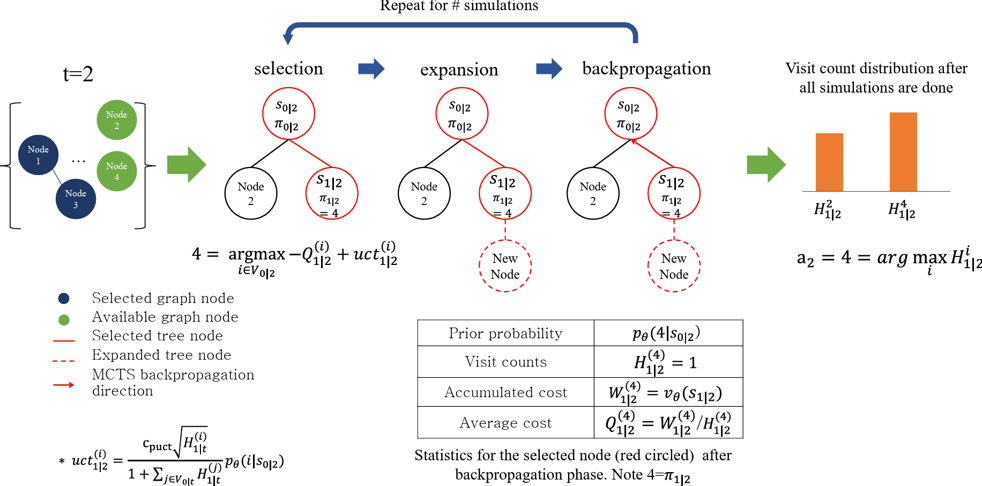
\includegraphics[width=0.94\linewidth]{figures/MCTS detail - fixed.png}
  \caption{An overall process of transition using MCTS. It depicts the situation when MCTS is run at $t=2$, and some simulation iterations are done. }
  \label{fig:MCTS}
\end{figure}

After the selection phase, the expansion phase starts, updating the MCTS tree by expanding new child nodes in $V_{\ell|t}$ at node $\pi_{\ell | t}$ and moving to the backpropagation phase. Note that in the early stages of the MCTS iterations, the tree may not have expanded enough to select a terminal node, meaning $V_{\ell|t} \neq \emptyset, \ell<T-t$. As the MCTS iteration further advances, the tree expands enough so that the final selected node, $\phi_{\ell|t}$, from the selection phase becomes the terminal node, $V_{\ell|t}=\emptyset, \ell=T-t$, meaning that the routing has ended with no available node to move on. In the latter case, the MCTS iteration still continues until it reaches $ns$ in order to explore a variety of possible node paths.

%When the expansion reaches the terminal node, we repeat the three phases until the MCTS iteration reaches $ns$.
%Despite the absence of new nodes in the expansion phase due to the terminal status, the accumulated costs and visit counts are continually updated through the backpropagation phase, as described below. This ongoing process introduces the possibility of generating different result outputs.

%At the end of the selection phase, a leaf node $s_{l|t}$ is always selected. The next step, expansion, is executed here.
%A set of new child nodes is expanded from $s_{l|t}$ and each node holds prior probability from the trained policy network $p_\theta(\cdot | s_{l|t})$. For example, a set of new child tree nodes, $\forall i \in V_{l|t}$, is appended to $s_{l|t}$. These child nodes can be selected in the selection phase of the next simulation iteration i.e., if $k$ is the leaf inner-step, $k=l$, in the next simulation iteration $l=k+1$ is possible as new child nodes are appended to the $s_{l|t}$.

Finally, in the backpropagation phase, tracing back $\boldsymbol{\pi}_{0:\ell | t}$, we update $H^{(i)}_{k|t}$ and $W^{(i)}_{k|t}$ for all selected tree nodes in $k \in [\ell, \ell-1, \cdots, 0]$ and
%, representing the \textit{tree nodes} in the reversed order of the selected path $\boldsymbol{s_{\ell|t}}$.
all selected customer nodes $i \in \boldsymbol{\pi}_{0:\ell|t}$. Specifically, the update follows the rule below:

%\begin{align}\label{eqn-backpropagation-update1}
%    & H^{(i)}_{k|t} = H^{(i)}_{k|t} + 1, \\
    %&W^{(i)}_{k|t} = \{
    %\begin{array}{ll}
    %     W^{(i)}_{k|t} + C([\boldsymbol{\pi}_{0,t-1}; \boldsymbol{\pi}_{0:\ell | t}]), &  \; \ell = T-t,\\
    %     W^{(i)}_{k|t} + v_\theta(\phi_{\ell|t}), &  \; \ell < T-t.
    %\end{array}
%\end{align}
\begin{align}\label{eqn-backpropagation-update1}
    H^{(i)}_{k|t} = H^{(i)}_{k|t} + 1,
\end{align}
\begin{align}\label{eqn-backpropagation-update2}
    W^{(i)}_{k|t} = \{
    \begin{array}{ll}
         W^{(i)}_{k|t} + C([\boldsymbol{\pi}_{0,t-1}; \boldsymbol{\pi}_{0:\ell | t}]), &  \; \ell = T-t,\\
         W^{(i)}_{k|t} + v_\theta(\phi_{\ell|t}), &  \; \ell < T-t.
    \end{array}
\end{align}

As the MCTS iteration continues, the selected leaf node can be either a terminal node ($\ell=T-t$), meaning that the routing has ended, or a non-terminal node ($\ell < T-t$). In the former case, $W^{(i)}_{k|t}$ accumulates the cost by evaluating the selected path of customer nodes, $C([\boldsymbol{\pi}_{0,t-1}; \boldsymbol{\pi}_{0:\ell | t}])$. However, in the latter, we use the predicted distance $v_\theta(\phi_{\ell|t})$. This is possible as we have trained the value network, $v_\theta(\cdot)$, to predict the final distance at any state following (eq. \ref{eqn:value_objective}).
In updating accumulated total cost, $W_{k|t}^{(i)}$, as in equation (\ref{eqn-backpropagation-update2}), we obtain the predicted cost by $v_\theta(\phi_{\ell|t})$ at the final selected node $\phi_{\ell|t}$, then greedily selecting the next customer node until the routing finishes. %with the maximum probability evaluated by $p_\theta(\cdot | s_{T-t | t})$.

%{\color{green}XX: %무슨 뜻인지 잘 이해가 안되는데, 한글로 설명을 커멘트로 넣어주어도 좋겠어요.
%Without the value network trained, when $\ell<T-t$, we need to temporarily finish the routing from the $\phi_{\ell|t}$ to obtain the cost to update the accumulated cost $W_{k|t}^{(i)}$. To finish the routing temporarily, we greedily select the next customer node until the routing finishes with the maximum probability evaluated by $p_\theta$, which is the same step as choosing the next customer node not using MCTS i.e., $\hat{a}_{k|t} = \argmax_{i \in V_{k|t}}{p_\theta(i|s_{k|t})}$. This requires several evaluations on the policy network for each MCTS simulation iteration, making the computation more heavy. We alleviate this problem by predicting the cost from $\phi_{\ell|t}$ using one evaluation of $v_\theta(\phi_{\ell|t})$.
%}
% 위의 내용은 다음과 같습니다. \ell < T-t인 경우에, Value network가 없는 경우라면, $W^{(i)}_{k|t}$를 업데이트 하기위해서 라우팅을 임시로 끝내야 합니다. 그래야만 최종 distance를 구할 수 있기 때문입니다. 따라서, 임시로 routing을 끝내기 위해서는 \phi_{\ell|t} 상태에서 k=[\ell, \ell+1, \cdots, T-t] level에 도달할 때까지 \argmax_{i \in V_{k|t}}{p_\theta(i|s_{k|t})}에 따라서 다음으로 이동할 customer node를 선택해서 움직여야 합니다. 즉, MCTS iteration 중에 backpropagation phase를 진행하기 위해서는 (value network가 없다면) 임시로 라우팅을 위에 적힌 식에 따라 끝내야 합니다. 당연히 해당 방법으로 routing을 끝내려면 여러번의 policy network가 실행되어야 합니다 (k=[\ell, \ell+1, \cdots, T-t]). 그러나, value network는 leaf node에서 최종적으로 얻게 될 distance를 예측할 수 있기 때문에, 굳이 임시로 routing을 끝낼 필요가 없어집니다. 임시로 routing을 끝낼 필요가 없어진다는 말은 다시 말해 policy network를 여러번 사용하여 routing을 수행할 필요가 없어진다는 의미입니다. 임시로 routing을 끝내는 과정은, MCTS의 메인 단계 (selection, expansion, backpropagtion)과는 다른, backpropagation을 할때만 수행이 되는 과정입니다.

When finishing all simulations, we collect a visit-count distribution from the $s_{0|t}$'s child nodes and choose the most visited node as $a_t$ for the next node to visit in the rollout:

\begin{align}\label{simulation result}
    & \pi_{t+1}=\hat{a}_t = \argmax_{i \in V_{0|t}} H^{(i)}_{1|t}.
\end{align}

% algorithm for MCTS simulation
\begin{algorithm}

\caption{Overall simulation flow in MCTS}\label{alg:simulation}
\begin{algorithmic}[1]
\Require $s_{0|t}$: root state initialized by $s_t$, $p_{\theta}$: trained policy network, $v_{\theta}$: trained value network, $ns$: number of simulations to run

\item[]
\State Initialize the MCTS tree by $s_{0|t}$
\While { $i < ns$}
    \State $\phi_{\ell|t}$,  $\boldsymbol{s}_{0:\ell|t}$,  $\boldsymbol{\pi}_{0:\ell|t}$ = \Call {Select}{$s_{0|t}$}   \Comment{A leaf node in the MCTS tree is chosen}

    \State \Call{Expand}{$p_\theta$, $\phi_{\ell|t}$}   \Comment{Expand the MCTS tree from the leaf node using available nodes $V_{\ell|t}$}

    \If{$V_{\ell|t} = \emptyset$} \Comment{The selection reached the terminal node}
        \State $c = C([\boldsymbol{\pi}_{0,t-1}; \boldsymbol{\pi}_{0:\ell | t}])$  \Comment{ (eq. \ref{eqn-backpropagation-update2})}

    \Else
        \State $c = v_\theta(\phi_{\ell|t})$   \Comment{Use the predicted cost for non-terminal leaf nodes}

    \EndIf

    \item[]

    \State \Call {Backpropagate}{$\boldsymbol{s}_{0:\ell|t}$, $c$}
    \State $i = i + 1$
    \item[]

\EndWhile

\State \Return $\argmax_{i \in V_{0|t}} H^{(i)}_{1|t}$

\end{algorithmic}
\end{algorithm}


Algorithm \ref{alg:simulation} summarizes the overall process of our MCTS. Additionally, the application of the MCTS is computationally expensive, making it impractical in real-usage. We found that most of $p_\theta(\cdot|s_t)$ outputs have low entropy, meaning the highest probability, $\max_{i} p_\theta(\cdot|s_t)$, dominates the other values. For example, we show the distribution of entropy values from $p_\theta(\cdot|s_t)$ in Figure \ref{fig:entropy_hist} of the experiment section.
Our idea is that we selectively apply our MCTS to the rollout when $\max_{i} p_\theta(\cdot|s_t)$ fails to dominate; that is to say when the difference between the highest probability and the fifth highest probability is less than $0.75$. We empirically obtained the strategy to improve the solution quality in trading the computation time off.

We present the pseudo-code for each MCTS phase in Algorithm \ref{alg:MCTS functions}.
We highlight the modifications made to adapt MCTS to the routing problems. Firstly, we applied min-max normalization to the Q-value calculated during the entire search phase.
%Q-value is the average distance observed on the node.
Since the Q-value ranges in $[0, \infty)$ which is equal to the range of cost (distance), this can cause a computational issue as the term $\frac{c_{puct}\sqrt{H^{(i)}_{k+1|t}}}{1 + H_{k+1|t}}p_{\theta(i| s_{k|t})}$ typically falls within range $[0, 1]$. Using a naive Q-value could lead to a heavy reliance on the Q-value when selecting the child node because of the scale difference.
%To mitigate this, we applied min-max normalization to the Q-values in the selection phase so that the normalized Q-value is in the range  $[0, 1]$. Note that
To apply min-max normalization to the Q-value in the implementation, we record the maximum and minimum values in the backpropagation phase.
Secondly, to minimize the distance, we negate the Q-value so that the search strategy aims to minimize distance. In the pseudo-code, STEP procedure, which we have not included in the paper due to its complexity, accepts the chosen action as input and processes the state to transit to the next state. Internally, we update the current position of the vehicle as the chosen action in addition to the current load of the vehicle if the problem is CVRP. In addition to it, the mask for unavailable nodes, $m_t$, is updated to prevent the vehicle from moving to visited nodes.

\begin{algorithm}
\caption{List of functions in MCTS}\label{alg:MCTS functions}

\begin{algorithmic}[1]
\Require $c_{puct}$=1.1: hyper-parmeter
\item[]

% select function
\Function{select}{$s_{0|t}$}
    \State $node \gets s_{0|t}$
    \State $\boldsymbol{s}_{0:\ell|t}$ = [$s_{0|t}$]
    \State $\boldsymbol{\pi}_{0:\ell|t}$ = [$\pi_{0|t}$]
    \State $k=0$

    \While{$node$ has child}
        \State $\pi_{k+1|t} = \argmax_{i \in V_{k|t}} -Q^{(i)}_{k+1|t} +  \frac{c_{\mbox{puct}} \sqrt{H^{(i)}_{k+1|t}}}{1 + \sum_{j\in V_{k|t}}H^{(j)}_{k+1|t}} p_{\theta}(i| s_{k|t})$   \Comment{(eq. \ref{selection expression})}
        \State Append $\pi_{k+1|t}$ to $\boldsymbol{\pi}_{0:\ell|t}$
        \State $node=s_{k+1|t}$ is updated with the child node selected
        \State Append $node$ to $\boldsymbol{s}_{0:\ell|t}$
        \State $k = k + 1$

    \EndWhile
    \State $\phi_{\ell|t} = node$ \Comment{Also, $\ell=k$}

\State \Return $\phi_{\ell|t}$,  $\boldsymbol{s}_{0:\ell|t}$,  $\boldsymbol{\pi}_{0:\ell|t}$
\EndFunction

\item[]

% expansion function
\Function{expand}{$p_\theta$, $\phi_{\ell|t}$}

\ForAll {$i \in V_{\ell|t}$}
    \State $s$, $cost$, $done$ = \Call {step}{$i$, $\phi_{\ell|t}$}  \Comment{Run STEP with the leaf node's state for the given $i$}
    \State create a new child node and assign $s$ as the state
    \State append the child node to $\phi_{\ell|t}$

\EndFor
\EndFunction
\item[]


\item[]

% Backpropagation function
\Function{backpropagate}{$\boldsymbol{s}_{0:\ell|t}$, $\boldsymbol{\pi}_{0:\ell|t}$, $c$}
    \State get [$\ell, \ell-1, \cdots, 0$] from $\boldsymbol{s}_{0:\ell|t}$
    \ForAll{$k$ $\in$ [$\ell, \ell-1, \cdots, 0$] and $i \in \boldsymbol{\pi}_{0:\ell|t}$} \Comment{$k$ denotes a level from the leaf to the root}
        \State $H_{k|t}^{(i)} \mathrel{+}= 1$
        \State $W_{k|t}^{(i)} \mathrel{+}= c$
        \State $Q_{k|t}^{(i)} = \frac{W_{k|t}^{(i)} }{H_{k|t}^{(i)}}$
        \State Normalize $Q_{k|t}^{(i)}$
    \EndFor
\EndFunction

\end{algorithmic}
\end{algorithm}

\section{Experiments}

At first, we generated problems by constructing $N$, the number of all nodes, random coordinates of which each coodinate is uniformly distributed in range $[0, 1]$. For CVRP, we assigned the first node as the depot node. In addition, we assigned the demand of each customer, $q_i$, with an integer between 1 to 10, scaled by 30, 40, 50 for the problem size ($n$) 20, 50, 100, respectively. We also applied POMO \cite{kwonPOMOPolicyOptimization2021} in our training, setting the pomo size as the number of customer nodes. However, in inference, we excluded POMO, as the utilization of MCTS is infeasible. Our implementation, available at the github\footnote{https://github.com/glistering96/AlphaRouter} url below, is built on Pytorch Lightning \cite{pytorchLightning} and Pytorch. \cite{paszke2017automatic}.
For the setting of MCTS, we set $c_{\mbox{puct}}$ as $1.1$, and varied the total number of simulations, $ns$,  by $100$, $500$, and $1000$. We measured the performance on 100 randomly generated problems as described above. For all the tables in this section, `dist' represents the average distance over all problems, and `time' represents the average inference time.


For the encoder and decoder settings, the size of each head's dimension is $32$ with $4$ heads, summed up to the embedding dimension, $d_e=128$, and $6$ encoder layers are used. We trained the model for $300$ epochs with batch size $64$, and $100000$ episodes. Note that this batch size plays as the number of parallel rollouts in training, meaning that $64$ episodes were simultaneously executed. We fixed the clipping parameter, $C$, to $10$. We used Adam \cite{kingma2014adam} with learning rate 1e-4, \textit{eps} 1e-7, and \textit{betas} $\in \{0.9, 0.95\}$ without any warm-up or schedulings. For fast training, we used 16-bit mixed precision.

We conducted the experiment on a machine equipped with i5-13600KF CPU, RTX 4080 16GB GPU, and 32GB RAM on Windows 11. For heuristic solvers in the experiment, we used the same machine except with a WSL setting on Ubuntu 22.04.

\subsection{Performance Comparison}

% Table generated by Excel2LaTeX from sheet 'TSP refined'
\begin{table}[htbp]
  \centering
  \caption{Results of TSP problems}
    \resizebox{\textwidth}{!}{
% Table generated by Excel2LaTeX from sheet 'TSP refined'
\begin{tabular}{c|c|c|c|c|c|c|c|c|c}
\toprule
\multicolumn{4}{c|}{Problem size ($n$)} & \multicolumn{2}{c|}{20} & \multicolumn{2}{c|}{50} & \multicolumn{2}{c}{100} \\
\midrule
Method & \multicolumn{1}{c|}{activation} & \multicolumn{1}{c|}{baseline} & $ns$     & \multicolumn{1}{c|}{dist} & \multicolumn{1}{c|}{time} & \multicolumn{1}{c|}{dist} & \multicolumn{1}{c|}{time} & \multicolumn{1}{c|}{dist} & \multicolumn{1}{c}{time} \\
\midrule
LKH3   & \multicolumn{3}{c|}{\multirow{4}[8]{*}{N.A.}} & \multicolumn{1}{c|}{3.8402 ± 0.05} & \multicolumn{1}{c|}{0.04± 0.01} & \multicolumn{1}{c|}{5.6705 ± 0.05} & \multicolumn{1}{c|}{0.411 ± 0.07} & \multicolumn{1}{c|}{7.7352 ± 0.05} & \multicolumn{1}{c}{1.167 ± 0.24} \\
\cmidrule{1-1}\cmidrule{5-10}OR Tools & \multicolumn{3}{c|}{}    & \multicolumn{1}{c|}{3.8402 ± 0.30} & \multicolumn{1}{c|}{  1.001 ± 0.00} & \multicolumn{1}{c|}{ 5.6807 ± 0.24} & \multicolumn{1}{c|}{ 1.00 ± 0.00} & \multicolumn{1}{c|}{ 7.9003 ± 0.28} & \multicolumn{1}{c}{ 7.001 ± 0.00} \\
\cmidrule{1-1}\cmidrule{5-10}\multicolumn{1}{p{4.565em}|}{Nearest \newline{}Insertions} & \multicolumn{3}{c|}{}    & \multicolumn{1}{c|}{4.3742 ± 0.08} & \multicolumn{1}{c|}{0.001 ± 0.00} & \multicolumn{1}{c|}{ 6.7550 ± 0.07} & \multicolumn{1}{c|}{ 0.00 ± 0.00} & \multicolumn{1}{c|}{ 9.4517 ± 0.08} & \multicolumn{1}{c}{ 0.003 ± 0.00} \\
\cmidrule{1-1}\cmidrule{5-10}Concorde & \multicolumn{3}{c|}{}    & \multicolumn{1}{c|}{3.8402 ± 0.05} & \multicolumn{1}{c|}{0.124 ± 0.03} & \multicolumn{1}{c|}{5.6705 ± 0.05} & \multicolumn{1}{c|}{1.292 ± 0.23} & \multicolumn{1}{c|}{7.7352 ± 0.05} & \multicolumn{1}{c}{5.143 ± 0.69} \\
\midrule
\midrule
\multicolumn{1}{c|}{\multirow{16}[8]{*}{DRL}} & \multicolumn{1}{c|}{\multirow{8}[4]{*}{ReLU}} & \multicolumn{1}{c|}{\multirow{4}[2]{*}{mean}} & 0      & 3.8492 ± 0.09 & 0.037 ± 0.00 & 5.7361 ± 0.06 & 0.079 ± 0.00 & 7.9852 ± 0.08 & 0.153 ± 0.00 \\
       &        &        & 100    & \textbf{3.8486 ± 0.09} & 0.043 ± 0.00 & 5.7375 ± 0.06 & 0.205 ± 0.01 & 7.9854 ± 0.08 & 0.627 ± 0.06 \\
       &        &        & 500    & 3.8491 ± 0.09 & 0.059 ± 0.00 & 5.7345 ± 0.06 & 0.592 ± 0.23 & 7.9826 ± 0.08 & 2.588 ± 1.82 \\
       &        &        & 1000   & 3.8491 ± 0.09 & 0.077 ± 0.01 & \textbf{5.7339 ± 0.06} & 1.051 ± 0.85 & \textbf{7.9807 ± 0.08} & 5.509 ± 9.14 \\
\cmidrule{3-10}       &        & \multicolumn{1}{c|}{\multirow{4}[2]{*}{val}} & 0      & 3.8489 ± 0.08 & 0.038 ± 0.00 & 5.7386 ± 0.06 & 0.078 ± 0.00 & 8.0481 ± 0.08 & 0.154 ± 0.00 \\
       &        &        & 100    & \textbf{3.8483 ± 0.08} & 0.038 ± 0.00 & 5.7310 ± 0.07 & 0.194 ± 0.01 & \textbf{8.0465 ± 0.08} & 0.648 ± 0.08 \\
       &        &        & 500    & \textbf{3.8483 ± 0.08} & 0.044 ± 0.00 & \textbf{5.7291 ± 0.07} & 0.533 ± 0.21 & 8.0687 ± 0.09 & 2.897 ± 2.03 \\
       &        &        & 1000   & \textbf{3.8483 ± 0.08} & 0.052 ± 0.01 & 5.7301 ± 0.06 & 0.959 ± 0.88 & 8.0564 ± 0.08 & 5.915 ± 9.45 \\
\cmidrule{2-10}       & \multicolumn{1}{c|}{\multirow{8}[4]{*}{SwiGLU}} & \multicolumn{1}{c|}{\multirow{4}[2]{*}{mean}} & 0      & 3.8464 ± 0.08 & 0.037 ± 0.00 & 5.7267 ± 0.07 & 0.080 ± 0.00 & 7.9562 ± 0.07 & 0.155 ± 0.00 \\
       &        &        & 100    & 3.8462 ± 0.08 & 0.045 ± 0.00 & \textbf{5.7248 ± 0.07} & 0.173 ± 0.01 & \textbf{7.9523 ± 0.07} & 0.594 ± 0.09 \\
       &        &        & 500    & \textbf{3.8461 ± 0.08} & 0.065 ± 0.01 & 5.7260 ± 0.07 & 0.458 ± 0.17 & 7.9530 ± 0.07 & 2.362 ± 2.72 \\
       &        &        & 1000   & \textbf{3.8461 ± 0.08} & 0.089 ± 0.02 & 5.7257 ± 0.07 & 0.799 ± 0.62 & 7.9539 ± 0.07 & 4.941 ± 13.23 \\
\cmidrule{3-10}       &        & \multicolumn{1}{c|}{\multirow{4}[2]{*}{val}} & 0      & 3.8482 ± 0.09 & 0.038 ± 0.00 & 5.7405 ± 0.07 & 0.081 ± 0.00 & 7.9551 ± 0.07 & 0.156 ± 0.00 \\
       &        &        & 100    & \textbf{3.8474 ± 0.09} & 0.047 ± 0.00 & 5.7377 ± 0.07 & 0.192 ± 0.01 & 7.9536 ± 0.07 & 0.646 ± 0.07 \\
       &        &        & 500    & 3.8478 ± 0.09 & 0.069 ± 0.01 & 5.7377 ± 0.07 & 0.550 ± 0.19 & 7.9630 ± 0.07 & 2.781 ± 1.93 \\
       &        &        & 1000   & 3.8478 ± 0.09 & 0.093 ± 0.02 & \textbf{5.7373 ± 0.07} & 0.961 ± 0.70 & \textbf{7.9522 ± 0.07} & 5.822 ± 9.99 \\
\bottomrule
\end{tabular}%
    }
  \label{tab:TSP result}%
\end{table}%


In this section, we compare the performance of the proposed MCTS-equipped model with that of some heuristics for the two routing problems, TSP and CVRP.
The baseline models for TSP are heuristic solvers, LKH3 \cite{helsgaunExtensionLinKernighanHelsgaunTSP}, Concorde \cite{applegateConcordeTspSolver2019}, Google's OR Tools \cite{ortools}, and Neareset Insertion strategy \cite{nearset_insertion}. These heuristic solvers, developed by optimization experts, serve as benchmarks for assessing optimization capabilities in solving routing problems. For Google's OR Tools, we added a guided-search  option, and the result reported here is better than the result reported in previous research \cite{kwonPOMOPolicyOptimization2021, kool2018attention}. For a fair comparison, the time limit for OR Tools is set to be similar to the longest MCTS runtime, $ns=1000$, for each $n$.

For comparison, additionally, we denote the proposed model without the MCTS strategy as an attention model (AM) that leverages solely the proposed neural network without MCTS. When integrating the MCTS strategy with the network model, we varied the number of simulations to investigate its impact on the performance. We evaluated one case using $100$ randomly generated by a same generation strategy employed during training. The comparative results of TSP and CVRP problems are summarized in Tables \ref{tab:TSP result} and  \ref{tab:CVRP result}, respectively. The column named $ns$ represents the number of simulations in the MCTS strategy, and $ns=0$ denotes the AM's result without the MCTS strategy. Thus, the `DRL' method includes the proposed method and the AM method. The column named `baseline' represents the different baseline $b(s)$ used in (\ref{eqn:gradient-of-policy-objective1}), in which "mean" represents the mean-over-batches baseline, and `value' represents the baseline with the value network, $v_\theta$. The baseline term here differs from the heuristic baselines reported in the tables. The best results in the experiment cases of the DRL methods are bold-faced.
%In the Tables, `dist' represents the average of tour distances $C(\boldsymbol{\pi}_{0,T})$, and `time' represents the average inference times to complete the tours.

\begin{table}[htbp]
  \centering
  \caption{CVRP problem result}
    \resizebox{\textwidth}{!}{
    % Table generated by Excel2LaTeX from sheet 'MCTS에 시간 맞춘 CVRP'
    \begin{tabular}{c|c|c|c|c|c|c|c|c|c}
    \toprule
    \multicolumn{4}{c|}{Problem size ($n$)} & \multicolumn{2}{c|}{20} & \multicolumn{2}{c|}{50} & \multicolumn{2}{c}{100} \\
    \midrule
    Method & activation & \multicolumn{1}{c|}{baseline} & \multicolumn{1}{c|}{$ns$} & \multicolumn{1}{c|}{dist} & \multicolumn{1}{c|}{time} & \multicolumn{1}{c|}{dist} & \multicolumn{1}{c|}{time} & \multicolumn{1}{c|}{dist} & \multicolumn{1}{c}{time} \\
    \midrule
    LKH3   & \multicolumn{3}{c|}{\multirow{2}[4]{*}{N.A.}} & \multicolumn{1}{c|}{6.1528 ± 0.16} & \multicolumn{1}{c|}{3.948 ± 0.46} & \multicolumn{1}{c|}{10.2951 ± 0.24} & \multicolumn{1}{c|}{14.617 ± 1.15} & \multicolumn{1}{c|}{15.4804 ± 0.33} & \multicolumn{1}{c}{26.03 ± 1.87} \\
    \cmidrule{1-1}\cmidrule{5-10}OR Tools & \multicolumn{3}{c|}{}    & \multicolumn{1}{c|}{6.2049 ± 0.85} & \multicolumn{1}{c|}{1.002 ± 0.00} & \multicolumn{1}{c|}{10.5973 ± 1.25} & \multicolumn{1}{c|}{5.000 ± 0.00} & \multicolumn{1}{c|}{16.273 ± 1.76} & \multicolumn{1}{c}{18.000 ± 0} \\
    \midrule
    \midrule
    \multicolumn{1}{c|}{\multirow{16}[8]{*}{DRL}} & \multicolumn{1}{c|}{\multirow{8}[4]{*}{ReLU}} & \multicolumn{1}{c|}{\multirow{4}[2]{*}{mean}} & 0      & 6.4097 ± 0.75 & 0.045 ± 0.00 & \textbf{10.8050 ± 1.65} & 0.095 ± 0.00 & 16.4418 ± 2.99 & 0.178 ± 0.00 \\
           &        &        & 100    & \textbf{6.4010 ± 0.76} & 0.151 ± 0.01 & 10.8225 ± 1.59 & 0.473 ± 0.03 & 16.4627 ± 3.00 & 1.326 ± 0.12 \\
           &        &        & 500    & 6.4065 ± 0.75 & 0.398 ± 0.13 & 10.8192 ± 1.60 & 1.737 ± 0.81 & 16.4596 ± 2.99 & 6.652 ± 3.91 \\
           &        &        & 1000   & 6.4073 ± 0.76 & 0.685 ± 0.45 & 10.8087 ± 1.63 & 3.258 ± 2.95 & \textbf{16.4387 ± 2.96} & 13.633 ± 17.61 \\
    \cmidrule{3-10}       &        & \multicolumn{1}{c|}{\multirow{4}[2]{*}{value}} & 0      & 6.4553 ± 0.80 & 0.046 ± 0.00 & \textbf{10.8634 ± 1.65} & 0.095 ± 0.00 & \textbf{16.4463 ± 3.00} & 0.177 ± 0.00 \\
           &        &        & 100    & 6.4452 ± 0.83 & 0.176 ± 0.01 & 10.8718 ± 1.61 & 0.466 ± 0.03 & 16.4750 ± 3.08 & 1.409 ± 0.13 \\
           &        &        & 500    & \textbf{6.4449 ± 0.84} & 0.489 ± 0.15 & 10.8651 ± 1.65 & 1.773 ± 0.78 & 16.4494 ± 3.02 & 7.079 ± 3.34 \\
           &        &        & 1000   & 6.4479 ± 0.80 & 0.831 ± 0.47 & 10.8774 ± 1.67 & 3.475 ± 3.65 & 16.4468 ± 2.98 & 14.504 ± 14.40 \\
    \cmidrule{2-10}       & \multicolumn{1}{c|}{\multirow{8}[4]{*}{SwiGLU}} & \multicolumn{1}{c|}{\multirow{4}[2]{*}{mean}} & 0      & 6.4231 ± 0.73 & 0.046 ± 0.00 & 10.7940 ± 1.70 & 0.097 ± 0.00 & \textbf{16.4043 ± 3.09} & 0.180 ± 0.00 \\
           &        &        & 100    & \textbf{6.4228 ± 0.75} & 0.141 ± 0.01 & \textbf{10.7747 ± 1.71} & 0.464 ± 0.05 & 16.4190 ± 3.10 & 1.243 ± 0.14 \\
           &        &        & 500    & 6.4230 ± 0.73 & 0.346 ± 0.08 & 10.7878 ± 1.72 & 1.742 ± 1.02 & 16.4169 ± 3.10 & 6.018 ± 4.62 \\
           &        &        & 1000   & 6.4292 ± 0.74 & 0.562 ± 0.23 & 10.7847 ± 1.67 & 3.260 ± 3.71 & 16.4117 ± 3.11 & 12.221 ± 20.71 \\
    \cmidrule{3-10}       &        & \multicolumn{1}{c|}{\multirow{4}[2]{*}{val}} & 0      & 6.4201 ± 0.72 & 0.046 ± 0.00 & 10.8402 ± 1.48 & 0.096 ± 0.00 & 16.3575 ± 3.04 & 0.178 ± 0.00 \\
           &        &        & 100    & \textbf{6.4020 ± 0.74} & 0.154 ± 0.01 & 10.8420 ± 1.53 & 0.517 ± 0.04 & 16.3950 ± 2.97 & 1.188 ± 0.11 \\
           &        &        & 500    & 6.4055 ± 0.73 & 0.422 ± 0.10 & \textbf{10.8336 ± 1.49} & 1.959 ± 1.02 & \textbf{16.3475 ± 3.05} & 5.671 ± 3.51 \\
           &        &        & 1000   & 6.4101 ± 0.72 & 0.686 ± 0.28 & 10.8456 ± 1.53 & 3.683 ± 3.64 & 16.3492 ± 3.02 & 11.610 ± 14.31 \\
    \bottomrule
    \end{tabular}%
    }
  \label{tab:CVRP result}%
\end{table}%

For TSP, none of the records from AM, denoted by $ns=0$, is bold-faced, meaning that the MCTS application improved the solution quality. For CVRP, some records using AM are bold but the best records are all from the cases with MCTS.
%Therefore, applying MCTS does help improve the solution quality.
We provide the visualization of the two different methods results in Figure \ref{fig:visualized result} for better understanding of the effectiveness of MCTS. Visually and quantitatively, the solution in Figure \ref{fig:visualized result}(b) by the proposed model is better than that in Figure \ref{fig:visualized result}(a) by the AM.

The results reveal that while the application of the MCTS contributes to performance enhancement compared to the ones without the MCTS, it still falls short of the performance achieved by the heuristic models as other research shows \cite{kwonPOMOPolicyOptimization2021, kool2018attention}. Contrary to our expectation, an increase in the number of simulations does not consistently lead to solution improvement, a decrease in distance. The analysis indicates a lack of a discernible relationship between the number of simulations and the resulting distance. Specifically, for problems with a size of $50$, Pearson's correlation coefficient between the two is $\mbox{-}0.72$, and for the case of CVRP with a size of $100$, it is $\mbox{-}0.47$. In other cases, correlation scores are generally low, below $0.2$.

\begin{figure}
    \begin{center}
        \begin{subfigure}[b]{0.49\linewidth}
        \centering
         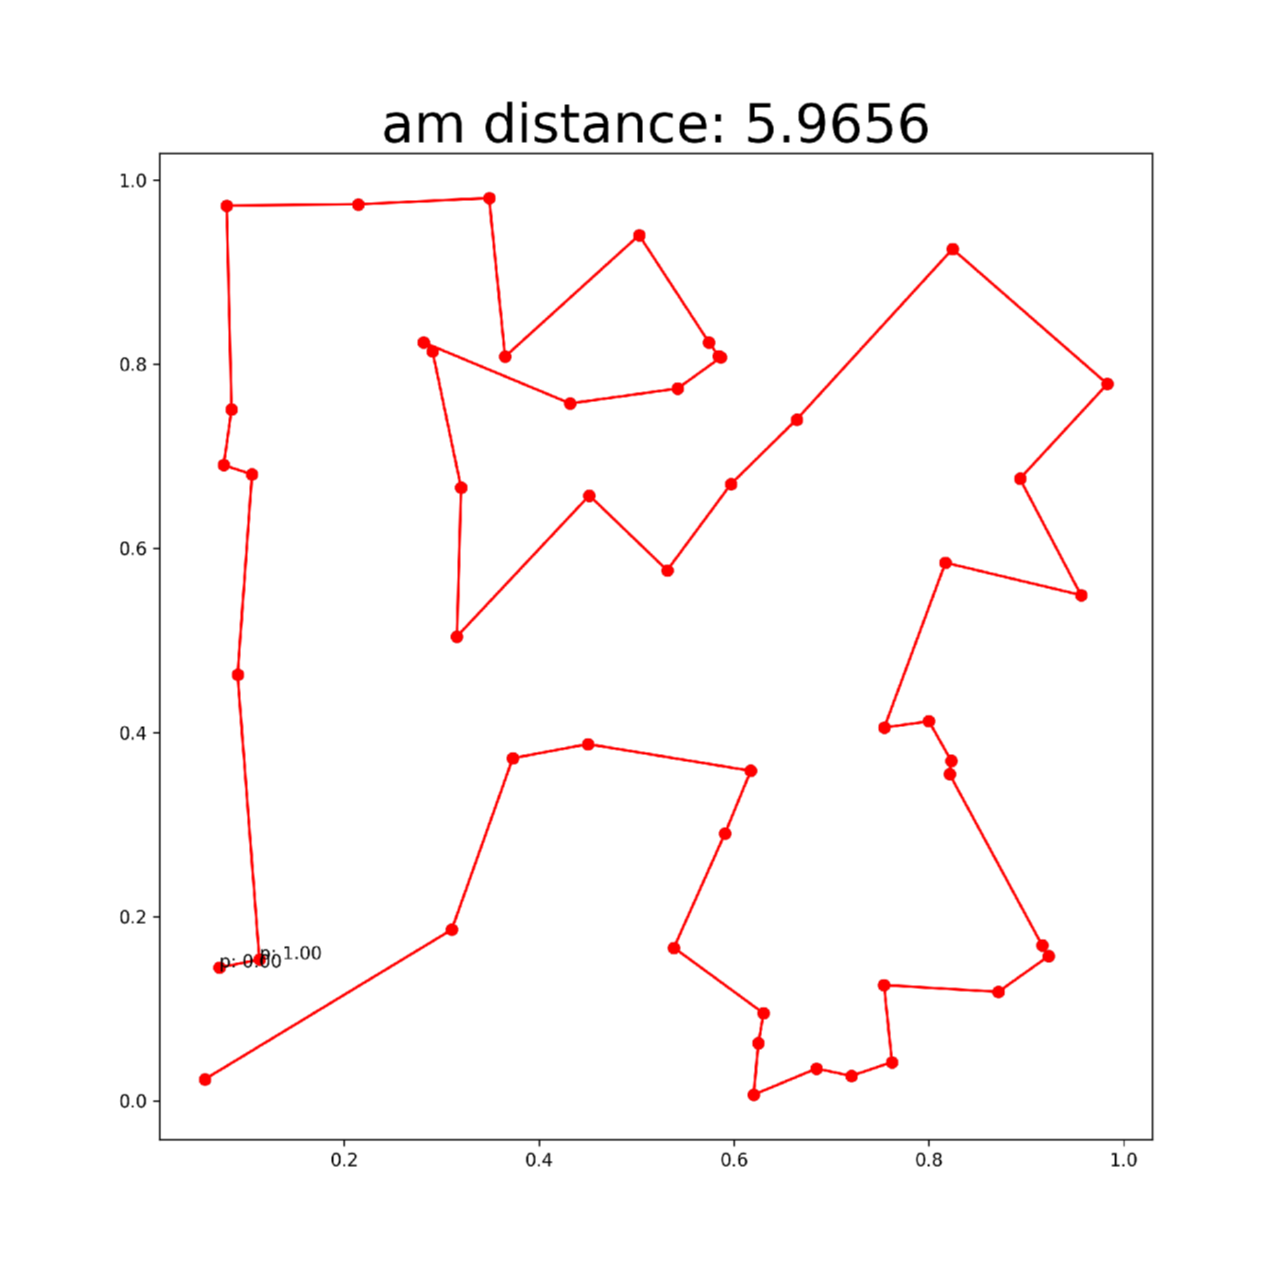
\includegraphics[width=\linewidth]{figures/AM result.png}
         \caption{Attention only model's result}
         \label{fig:AM-result}
        \end{subfigure}
        \hfill
        \begin{subfigure}[b]{0.49\linewidth}
            \centering
             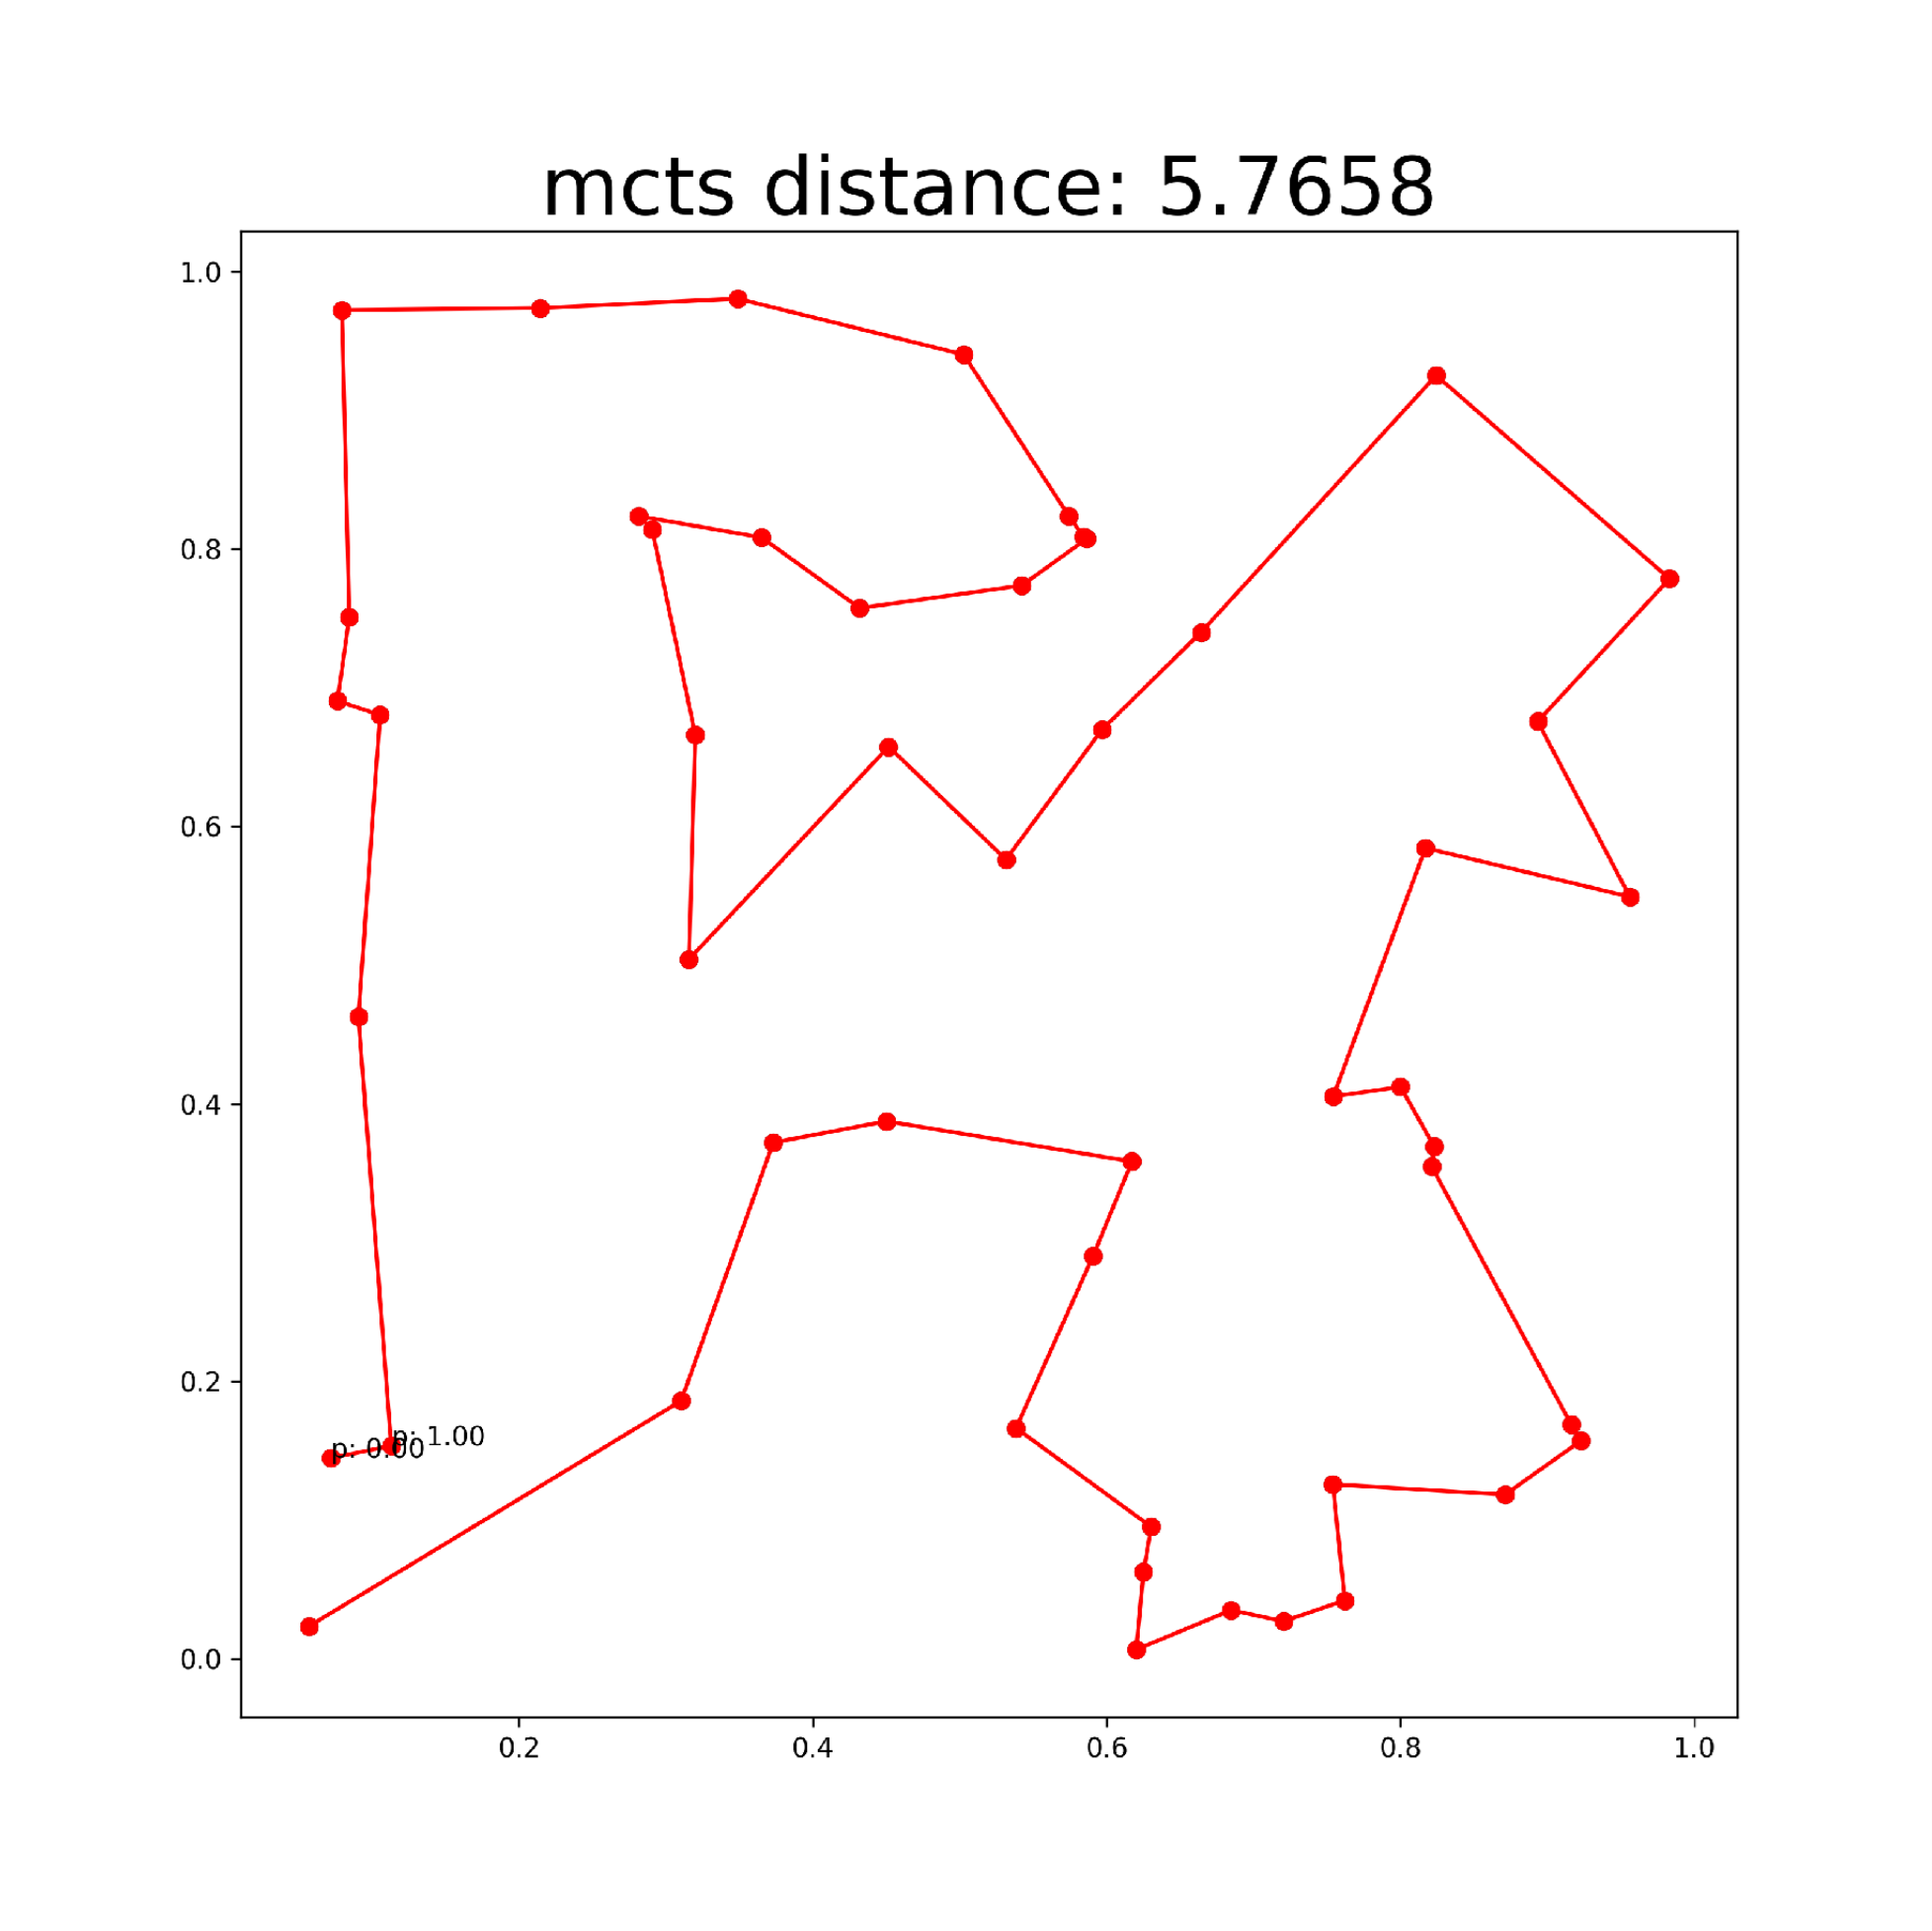
\includegraphics[width=\linewidth]{figures/MCTS result.png}
             \caption{MCTS applied model's result}
             \label{fig:MCTS-result}
        \end{subfigure}
    \end{center}
    \caption{Visualization of two methods' resutls on the same test data}
    \label{fig:visualized result}
\end{figure}

In addition, the MCTS strategy induces a small runtime overhead compared to the method without MCTS, AM. For CVRP problems, the average runtimes of the proposed method are considerably shorter than those of the LKH3 method. However, the runtime increases according to the problem size $n$. Our explanation is that, as the problem gets bigger, some large problems are hard to solve only by the probability outputs from $p_\theta$, therefore utilizing MCTS more. We argue that to improve the solution quality of AM, numerous samples of solutions, which take a huge amount of time to generate, are required. This result is also shown in the experiment results from \cite{kwonPOMOPolicyOptimization2021}. Also, we point out that training the network with more learning epochs to lower a small amount of distance takes quite a long time. For example, to lower about $0.015$ in distance by training the network after $300$ epochs, we need approximately $24$ hours as described in Figure \ref{fig:time-to-train} in which the orange line is the regressed line over the observations. However, with MCTS, we can consistently get better solution results within a few seconds and the method is deterministic, unlike sampling methods. Nonetheless, we believe there still is room for improving the runtime of MCTS. The heuristic solvers were written in C while our MCTS is written in Python, which is very slow. Implementing MCTS in C++ with parallelism should decrease the runtime much more than now.


\begin{figure}
    \centering
    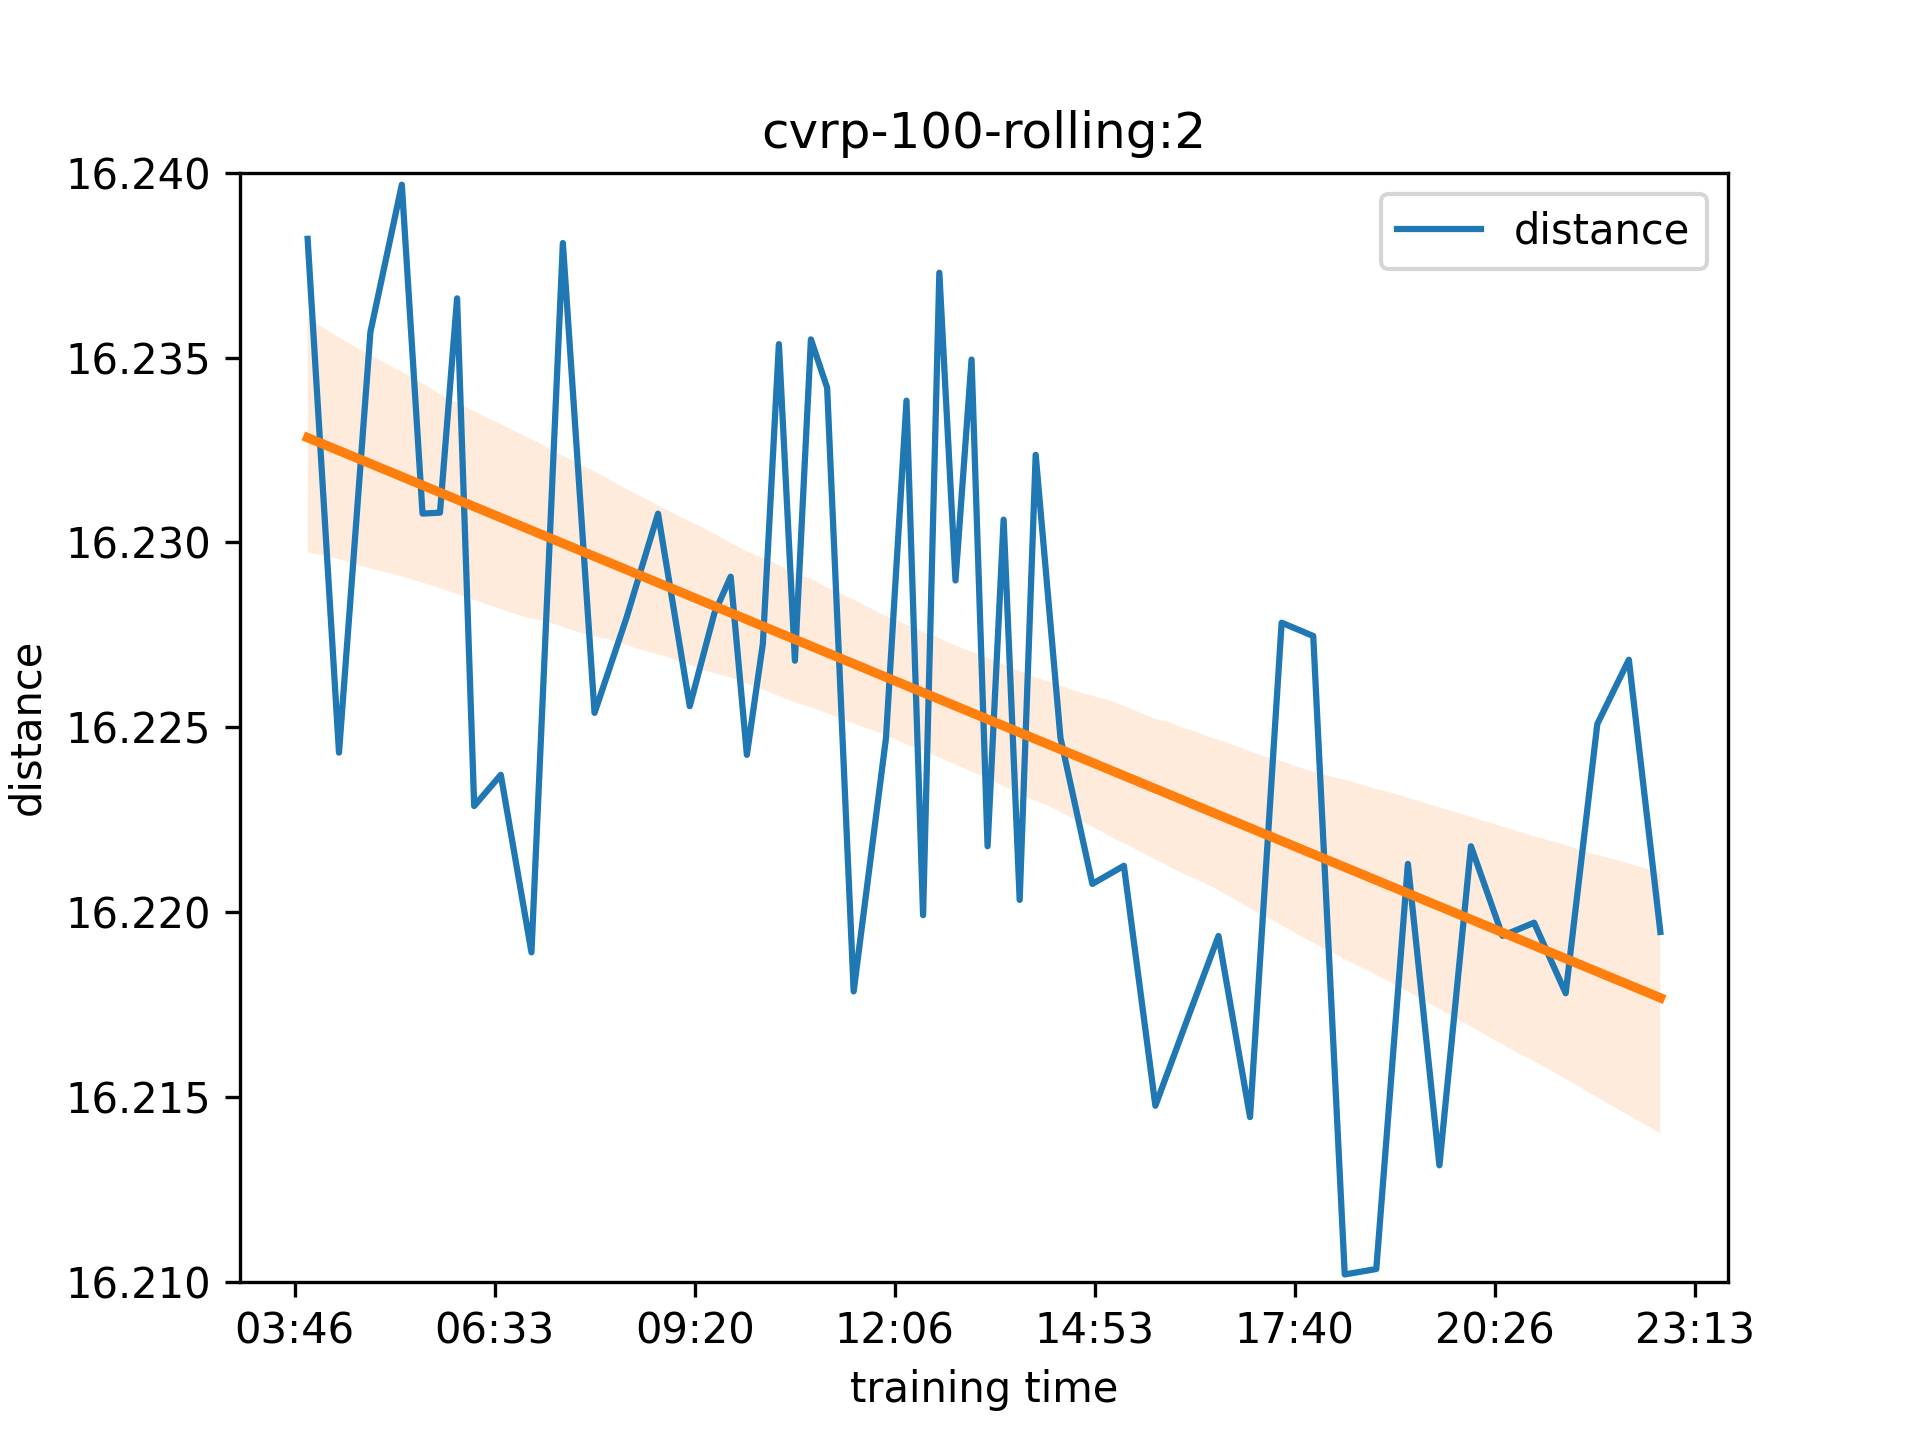
\includegraphics[width=0.75\linewidth]{figures/cvrp-100-rolling_2.png}
    \caption{Training score after 300 epochs on CVRP-100 problem smoothed on the window size 2.}
    \label{fig:time-to-train}
\end{figure}


% Table generated by Excel2LaTeX from sheet 'paired t-test result'
\begin{table}[htbp]
  \centering
  \caption{t-test report within the same conditions}
  \resizebox{\textwidth}{!}{
\begin{tabular}{c|c|cc|c|c|}
\toprule
problem type & problem size & AM     & MCTS   & p-value & <0.05 \\
\midrule
\midrule
\multirow{3}[2]{*}{tsp} & 20     & SwiGLU-val & SwiGLU-val-100 & 0.1    & FALSE \\
       & 50     & ReLU-val & ReLU-val-500 & 0.0144 & TRUE \\
       & 100    & ReLU-mean & ReLU-mean-1000 & 0.0262 & TRUE \\
\midrule
\multirow{3}[2]{*}{cvrp} & 20     & SwiGLU-val & SwiGLU-val-1000 & 0.0066 & TRUE \\
       & 50     & SwiGLU-mean & SwiGLUe-mean-100 & 0.0994 & FALSE \\
       & 100    & SwiGLU-val & SwiGLU-val-100 & 0.0339 & TRUE \\
\bottomrule
\end{tabular}%

    }
  \label{tab:t-test-same-components}%
\end{table}%

% Table generated by Excel2LaTeX from sheet 'paired t-test result'
\begin{table}[htbp]
  \centering
  \caption{t-test report regardless of the conditions}
  \resizebox{\textwidth}{!}{
\begin{tabular}{c|c|cc|c|c|}
\toprule
problem type & problem size & AM     & MCTS   & p-value & <0.05 \\
\midrule
\midrule
\multirow{3}[2]{*}{tsp} & 20     & SwiGLU-val & SwiGLU-val-100 & 0.1    & FALSE \\
       & 50     & ReLU-val & ReLU-val-500 & 0.0144 & TRUE \\
       & 100    & ReLU-val & SwiGLU-mean-100 & 0.0001 & TRUE \\
\midrule
\multirow{3}[2]{*}{cvrp} & 20     & SwiGLU-val & SwiGLU-val-1000 & 0.0066 & TRUE \\
       & 50     & ReLU-val & SwiGLUe-mean-100 & 0.0064 & TRUE \\
       & 100    & SwiGLU-val & ReLU-mean-100 & 0.0056 & TRUE \\
\bottomrule
\end{tabular}%

    }
  \label{tab:t-test-not-same-components}%
\end{table}%

To statistically confirm the effectiveness of the proposed MCTS, we include paired t-test results for two different cases. Table \ref{tab:t-test-same-components} reports the test results within the same conditions such as activation function and baselines. The records in the AM column follow the format "activation-baseline" and the records in the MCTS column follow "activation-baseline-MCTS simulation number". In this setting, the test shows that applying the MCTS improves the solution than without the MCTS except for TSP-20 and CVRP-50. We suspect that for relatively small size problems, relying on policy network only (AM) can be good enough but if the problem gets bigger, introducing the MCTS can result in better solutions.
On the other hand, Table \ref{tab:t-test-not-same-components} shows the test results regardless of the conditions, so that we report the lowest p-value for each problem type and size. It implies that the application of the MCTS is worth for a given problem type even if the change of activation and baseline is allowed.

We also show the entropy of $p_\theta(\cdot)$ for all test cases in TSP with size $100$ in Figure \ref{fig:entropy_hist}. We found that $86$\% of entropies are below $0.1$, meaning that the outcomes of $p_\theta(\cdot)$ are dominated by a few suggestions and a mere application of $p_\theta(\cdot)$ might lead to local optimal. Therefore, while controling time overhead, applying MCTS selectively is a good strategy. We show the evaluation result for not applying MCTS selectively in the Ablation analysis in the next subsection.

\begin{figure}
    \centering
    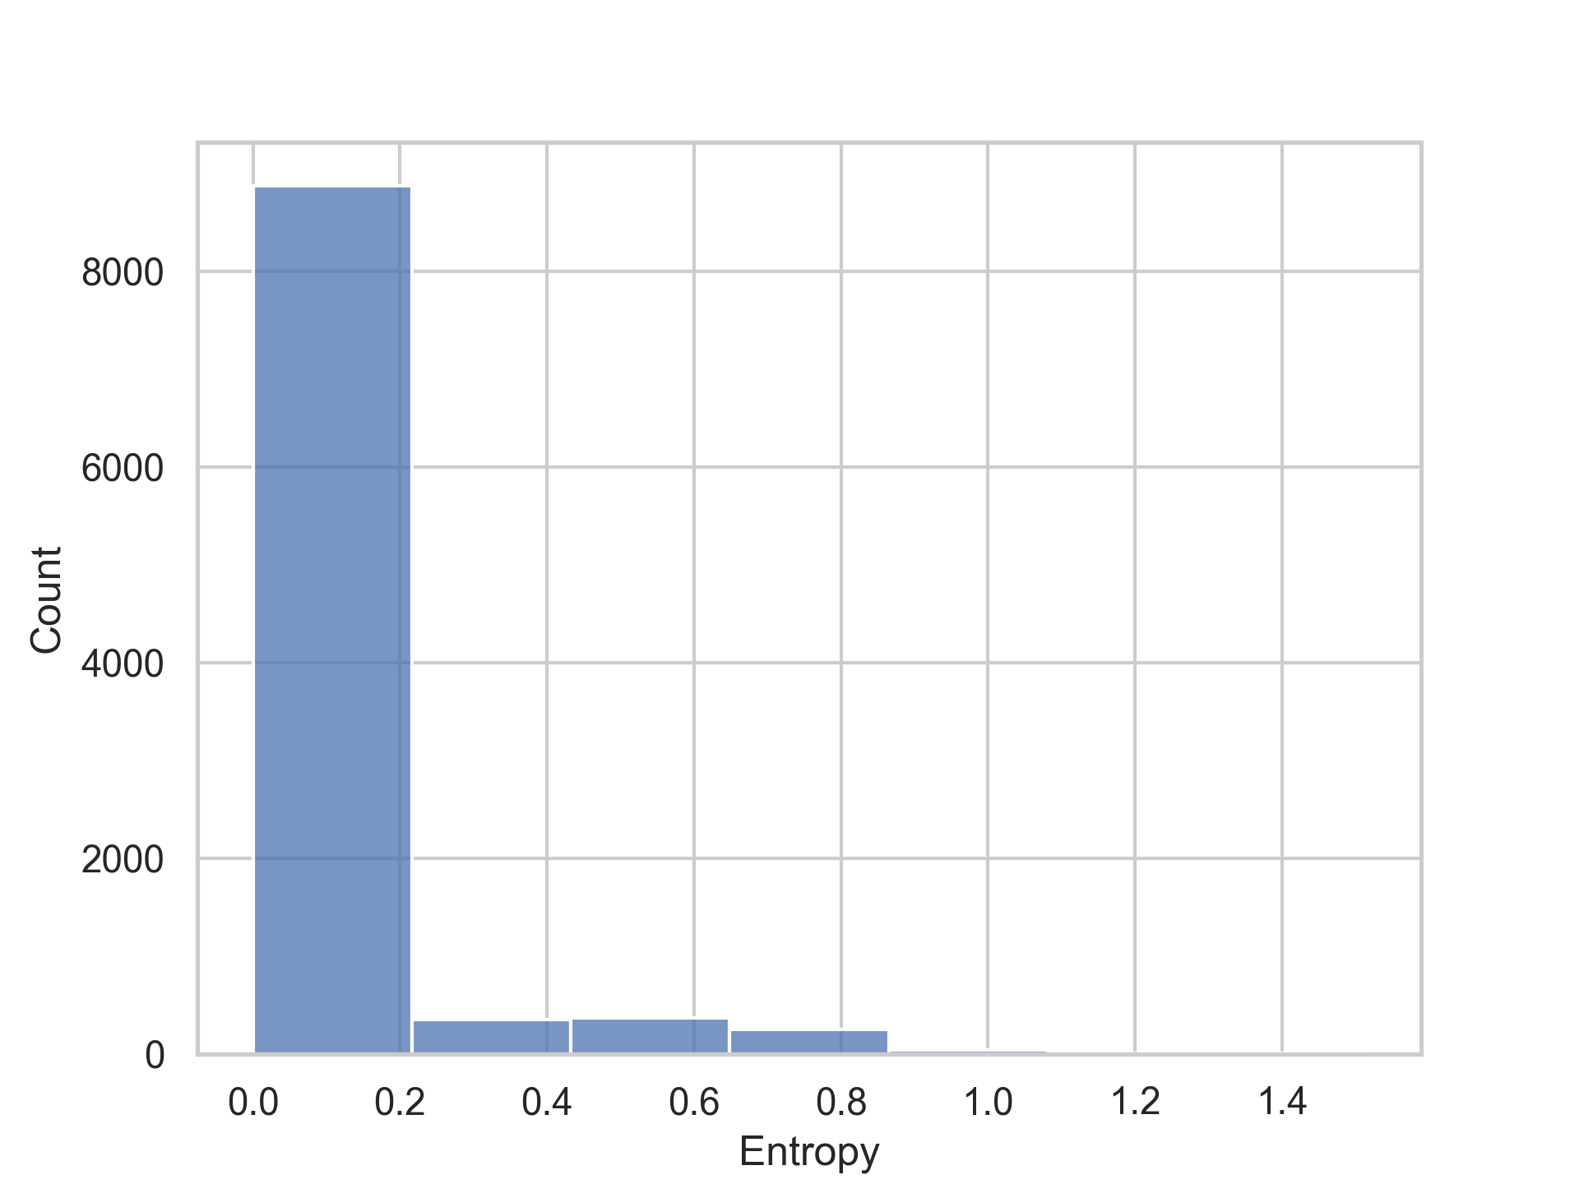
\includegraphics[width=0.5\linewidth]{figures/entropy.png}
    \caption{Histogram of entropies of policy network $p_\theta(\cdot)$ for TSP with size $100$}
    \label{fig:entropy_hist}
\end{figure}

\subsection{Ablation analysis}

In this section, we present some ablation results for the activation function and the baseline. We aggregated the results based on the activation function used and then calculated the mean and standard deviation of the score over all settings, i.e., AM, MCTS-100, MCTS-500, MCTS-1000, and the result is described in Table \ref{tab: activation}.

% Table generated by Excel2LaTeX from sheet 'activation'
\begin{table}[htbp]
  \centering
  \caption{Performance results according to activation functions}
    \resizebox{\textwidth}{!}{
    % Table generated by Excel2LaTeX from sheet 'activation'
    \begin{tabular}{c|c|c|c|c|c|c|c}
    \toprule
    \multicolumn{1}{c}{\textbf{problem}} & \textbf{size} & \multicolumn{2}{c|}{\textbf{20}} & \multicolumn{2}{c|}{\textbf{50}} & \multicolumn{2}{c}{\textbf{100}} \\
    \cmidrule{2-8}\textbf{type} & \textbf{activation} & \textbf{score} & \textbf{runtime} & \textbf{score} & \textbf{runtime} & \textbf{score} & \textbf{runtime} \\
    \midrule
    \midrule
    \multirow{2}[2]{*}{\textbf{TSP}} & \textbf{ReLU} & 3.8487 ± 0.09 & 0.049 ± 0.00 & 5.7338 ± 0.06 & 0.462 ± 0.27 & 8.0192 ± 0.08 & 2.312 ± 2.82 \\
          & \textbf{SwiGLU} & \textbf{3.8470 ± 0.08} & 0.060 ± 0.01 & \textbf{5.7321 ± 0.07} & 0.412 ± 0.21 & \textbf{7.9549 ± 0.07} & 2.182 ± 3.50 \\
    \midrule
    \multirow{2}[2]{*}{\textbf{CVRP}} & \textbf{ReLU} & 6.4272 ± 0.79 & 0.353 ± 0.15 & 10.8416 ± 1.63 & 1.421 ± 1.03 & 16.4526 ± 3.00 & 5.620 ± 4.94 \\
          & \textbf{SwiGLU} & \textbf{6.4170 ± 0.73} & 0.300 ± 0.09 & \textbf{10.8128 ± 1.60} & 1.477 ± 1.18 & \textbf{16.3876 ± 3.06} & 4.789 ± 5.43 \\
    \bottomrule
    \end{tabular}%


    }
  \label{tab: activation}%
\end{table}%

We can easily see that as the problem size gets bigger, SwiGLU scores shorter distances overall than ReLU. Also, we noticed that as the problem size gets bigger, the difference between ReLU and SwiGLU is more apparent. For example, for CVRP problem types, when the problem size is n=20, the difference of the distances is about 0.01 while the number gets bigger $n$=100, by reaching up to around 0.07. The scalability of SwiGLU is much better than ReLU.

For the baseline, we have suggested two different approaches: mean over batches and value-net-based approach. This baseline is used in (\ref{eqn:gradient-of-policy-objective1}) as $b(s)$. We calculated the mean and standard deviation of the distances over all settings based on the type of baseline used, like we did in the activation function analysis and the result is described in Table \ref{tab: baseline}. Surprisingly, the mean baseline approach dominates over the value net baseline except for CVRP with problem size 100, which is the hardest problem in the settings. We presume that if the problem becomes complex, the value net baseline may perform better than the mean baseline. For instance, CVRP with a time window and pick-up may be solved better with the value net baseline.

% Table generated by Excel2LaTeX from sheet 'baseline'
\begin{table}[htbp]
  \centering
  \caption{Aggregated results of baselines}
    \resizebox{\textwidth}{!}{
        % Table generated by Excel2LaTeX from sheet 'baseline'
        \begin{tabular}{c|c|c|c|c|c|c|c}
        \toprule
        \multicolumn{1}{c}{\textbf{problem}} & \textbf{size} & \multicolumn{2}{c|}{\textbf{20}} & \multicolumn{2}{c|}{\textbf{50}} & \multicolumn{2}{c}{\textbf{100}} \\
        \cmidrule{2-8}\textbf{type} & \textbf{baseline} & \textbf{score} & \textbf{runtime} & \textbf{score} & \textbf{runtime} & \textbf{score} & \textbf{runtime} \\
        \midrule
        \midrule
        \multirow{2}[2]{*}{\textbf{TSP}} & \textbf{mean} & \textbf{3.8476 ± 0.09} & 0.057 ± 0.01 & \textbf{5.7306 ± 0.06} & 0.429 ± 0.24 & \textbf{7.9687 ± 0.08} & 2.116 ± 3.38 \\
              & \textbf{value} & 3.8481 ± 0.08 & 0.052 ± 0.00 & 5.7352 ± 0.07 & 0.444 ± 0.25 & 8.0054 ± 0.08 & 2.378 ± 2.94 \\
        \midrule
        \multirow{2}[2]{*}{\textbf{CVRP}} & \textbf{mean} & \textbf{6.4153 ± 0.75} & 0.297 ± 0.11 & \textbf{10.7996 ± 1.66} & 1.391 ± 1.07 & 16.4319 ± 3.04 & 5.181 ± 5.89 \\
              & \textbf{value} & 6.4289 ± 0.77 & 0.356 ± 0.13 & 10.8549 ± 1.57 & 1.508 ± 1.15 & \textbf{16.4083 ± 3.02} & 5.227 ± 4.48 \\
        \bottomrule
        \end{tabular}%

    }
  \label{tab: baseline}%
\end{table}%

 We also report the non-selective MCTS experiment results here. The authors should be aware that the hardware environment here is a little different from the result in the experiment section. For non-selective MCTS, we have run the experiment on a workstation shared among others that runs on Linux with RTX 4090 24GB and Intel Xeon w7-2475X. Therefore, the runtime recorded in the tables below cannot be directly compared to the result from the table from the experiment, but we still include them to observe the trend in the runtime. Despite different hardware settings and computing settings, we still believe that the difference in runtime between selective MCTS and non-selective MCTS is huge enough to support that selective MCTS is meaningful.

% Table generated by Excel2LaTeX from sheet 'TSP non-selective MCTS'
\begin{table}[htbp]
  \centering
  \caption{Non-selective MCTS applied on TSP}
  \resizebox{\textwidth}{!}{
    \begin{tabular}{c|c|c|c|c|c|c|c|c|c}
    \toprule
    \multicolumn{4}{c|}{Problem size} & \multicolumn{2}{c|}{20} & \multicolumn{2}{c|}{50} & \multicolumn{2}{c}{100} \\
    \midrule
    Method & \multicolumn{1}{c|}{activation} & \multicolumn{1}{c|}{baseline} & ns     & \multicolumn{1}{c|}{dist} & \multicolumn{1}{c|}{time} & \multicolumn{1}{c|}{dist} & \multicolumn{1}{c|}{time} & \multicolumn{1}{c|}{dist} & \multicolumn{1}{c}{time} \\
    \midrule
    LKH3   & \multicolumn{3}{c|}{\multirow{4}[8]{*}{N.A.}} & \multicolumn{1}{c|}{3.8402 ± 0.05} & \multicolumn{1}{c|}{0.04± 0.01} & \multicolumn{1}{c|}{5.6705 ± 0.05} & \multicolumn{1}{c|}{0.411 ± 0.07} & \multicolumn{1}{c|}{7.7352 ± 0.05} & \multicolumn{1}{c}{1.167 ± 0.24} \\
\cmidrule{1-1}\cmidrule{5-10}    OR Tools & \multicolumn{3}{c|}{}    & \multicolumn{1}{c|}{3.8402 ± 0.30} & \multicolumn{1}{c|}{ 5.001 ± 0.00} & \multicolumn{1}{c|}{ 5.6807 ± 0.24} & \multicolumn{1}{c|}{ 5.00 ± 0.00} & \multicolumn{1}{c|}{ 7.9154 ± 0.28} & \multicolumn{1}{c}{ 5.001 ± 0.00} \\
\cmidrule{1-1}\cmidrule{5-10}    \multicolumn{1}{p{4.565em}|}{Neareset \newline{}Insertions} & \multicolumn{3}{c|}{}    & \multicolumn{1}{c|}{4.3742 ± 0.08} & \multicolumn{1}{c|}{0.001 ± 0.00} & \multicolumn{1}{c|}{ 6.7550 ± 0.07} & \multicolumn{1}{c|}{ 0.00 ± 0.00} & \multicolumn{1}{c|}{ 9.4517 ± 0.08} & \multicolumn{1}{c}{ 0.003 ± 0.00} \\
\cmidrule{1-1}\cmidrule{5-10}    Concorde & \multicolumn{3}{c|}{}    & \multicolumn{1}{c|}{3.8402 ± 0.05} & \multicolumn{1}{c|}{0.124 ± 0.03} & \multicolumn{1}{c|}{5.6705 ± 0.05} & \multicolumn{1}{c|}{1.292 ± 0.23} & \multicolumn{1}{c|}{7.7352 ± 0.05} & \multicolumn{1}{c}{5.143 ± 0.69} \\
    \midrule
    \midrule
    \multicolumn{1}{c|}{\multirow{16}[8]{*}{DRL}} & \multicolumn{1}{c|}{\multirow{8}[4]{*}{ReLU}} & \multicolumn{1}{c|}{\multirow{4}[2]{*}{mean}} & 0      & 3.8492 ± 0.09 & 0.107 ± 0.00 & 5.7361 ± 0.06 & 0.231 ± 0.00 & 7.9852 ± 0.08 & 0.450 ± 0.00 \\
           &        &        & 100    & \textbf{3.8491 ± 0.09} & 0.864 ± 0.03 & \textbf{5.7356 ± 0.06} & 4.614 ± 0.55 & \textbf{7.9817 ± 0.08} & 10.342 ± 2.31 \\
           &        &        & 500    & \textbf{3.8491 ± 0.09} & 3.079 ± 0.25 & 5.7365 ± 0.06 & 17.099 ± 2.76 & 7.9855 ± 0.08 & 55.007 ± 24.24 \\
           &        &        & 1000   & \textbf{3.8491 ± 0.09} & 5.727 ± 0.34 & 5.7360 ± 0.06 & 31.821 ± 5.26 & 7.9848 ± 0.08 & 110.943 ± 76.95 \\
\cmidrule{3-10}           &        & \multicolumn{1}{c|}{\multirow{4}[2]{*}{value}} & 0      & 3.8489 ± 0.08 & 0.111 ± 0.00 & 5.7386 ± 0.06 & 0.230 ± 0.00 & 8.0481 ± 0.08 & 0.451 ± 0.00 \\
           &        &        & 100    & 3.8489 ± 0.08 & 0.879 ± 0.07 & \textbf{5.7294 ± 0.07} & 4.450 ± 0.60 & 8.0459 ± 0.08 & 9.434 ± 3.04 \\
           &        &        & 500    & \textbf{3.8483 ± 0.08} & 2.962 ± 0.08 & 5.7362 ± 0.06 & 16.844 ± 3.02 & \textbf{8.0453 ± 0.08} & 56.209 ± 35.65 \\
           &        &        & 1000   & \textbf{3.8483 ± 0.08} & 5.715 ± 0.28 & 5.7314 ± 0.07 & 31.341 ± 4.81 & 8.0456 ± 0.08 & 112.687 ± 105.85 \\
\cmidrule{2-10}           & \multicolumn{1}{c|}{\multirow{8}[4]{*}{SwiGLU}} & \multicolumn{1}{c|}{\multirow{4}[2]{*}{mean}} & 0      & 3.8464 ± 0.08 & 0.110 ± 0.00 & 5.7267 ± 0.07 & 0.237 ± 0.00 & 7.9562 ± 0.07 & 0.454 ± 0.00 \\
           &        &        & 100    & 3.8463 ± 0.08 & 0.940 ± 0.13 & \textbf{5.7263 ± 0.07} & 4.292 ± 0.38 & \textbf{7.9528 ± 0.07} & 10.239 ± 3.44 \\
           &        &        & 500    & \textbf{3.8459 ± 0.08} & 2.979 ± 0.12 & 5.7266 ± 0.07 & 16.516 ± 1.83 & 7.9542 ± 0.07 & 56.392 ± 29.80 \\
           &        &        & 1000   & 3.8461 ± 0.08 & 5.716 ± 0.32 & 5.7265 ± 0.07 & 30.746 ± 2.69 & 7.9542 ± 0.07 & 112.849 ± 84.50 \\
\cmidrule{3-10}           &        & \multicolumn{1}{c|}{\multirow{4}[2]{*}{value}} & 0      & 3.8482 ± 0.09 & 0.113 ± 0.00 & 5.7405 ± 0.07 & 0.234 ± 0.00 & 7.9551 ± 0.07 & 0.456 ± 0.00 \\
           &        &        & 100    & \textbf{3.8481 ± 0.09} & 0.860 ± 0.04 & 5.7403 ± 0.07 & 4.429 ± 0.45 & \textbf{7.9509 ± 0.07} & 10.046 ± 3.79 \\
           &        &        & 500    & 3.8481 ± 0.09 & 3.040 ± 0.16 & \textbf{5.7391 ± 0.07} & 16.917 ± 2.96 & 7.9516 ± 0.07 & 55.425 ± 39.04 \\
           &        &        & 1000   & 3.8481 ± 0.09 & 5.705 ± 0.27 & \textbf{5.7391 ± 0.07} & 31.496 ± 4.65 & 7.9516 ± 0.07 & 111.637 ± 113.14 \\
    \bottomrule
    \end{tabular}%
    }
  \label{tab:non-selective MCTS TSP}%
\end{table}%

 We can see that compared to the selective MCTS results from Table \ref{tab:TSP result}, a huge amount of runtime is required for MCTS. Also, the bolded record for each group is almost the same or a little bit better with the selective MCTS strategy.

 % Table generated by Excel2LaTeX from sheet 'CVRP non-selective MCTS'
\begin{table}[htbp]
  \centering
  \caption{Non-selective MCTS applied on CVRP}
  \resizebox{\textwidth}{!}{
    \begin{tabular}{c|c|c|c|c|c|c|c|c|c}
    \toprule
    \multicolumn{4}{c|}{Problem size} & \multicolumn{2}{c|}{20} & \multicolumn{2}{c|}{50} & \multicolumn{2}{c}{100} \\
    \midrule
    Method & activation & \multicolumn{1}{c|}{baseline} & \multicolumn{1}{c|}{ns} & \multicolumn{1}{c|}{dist} & \multicolumn{1}{c|}{time} & \multicolumn{1}{c|}{dist} & \multicolumn{1}{c|}{time} & \multicolumn{1}{c|}{dist} & \multicolumn{1}{c}{time} \\
    \midrule
    LKH3   & \multicolumn{3}{c|}{\multirow{2}[4]{*}{N.A.}} & \multicolumn{1}{c|}{6.1528 ± 0.16} & \multicolumn{1}{c|}{3.948 ± 0.46} & \multicolumn{1}{c|}{10.2951 ± 0.24} & \multicolumn{1}{c|}{14.617 ± 1.15} & \multicolumn{1}{c|}{15.4804 ± 0.33} & \multicolumn{1}{c}{26.03 ± 1.87} \\
\cmidrule{1-1}\cmidrule{5-10}    OR Tools & \multicolumn{3}{c|}{}    & \multicolumn{1}{c|}{6.2049 ± 0.85} & \multicolumn{1}{c|}{1.002 ± 0.00} & \multicolumn{1}{c|}{10.5973 ± 1.25} & \multicolumn{1}{c|}{5.000 ± 0.00} & \multicolumn{1}{c|}{16.273 ± 1.76} & \multicolumn{1}{c}{18.000 ± 0} \\
    \midrule
    \midrule
    \multicolumn{1}{c|}{\multirow{16}[8]{*}{DRL}} & \multicolumn{1}{c|}{\multirow{8}[4]{*}{ReLU}} & \multicolumn{1}{c|}{\multirow{4}[2]{*}{mean}} & 0      & 6.4097 ± 0.75 & 0.131 ± 0.00 & \textbf{10.8050 ± 1.65} & 0.279 ± 0.00 & 16.4418 ± 2.99 & 0.523 ± 0.00 \\
           &        &        & 100    & \textbf{6.4048 ± 0.77} & 1.067 ± 0.16 & 10.8133 ± 1.60 & 3.444 ± 0.57 & 16.4840 ± 3.06 & 6.453 ± 2.58 \\
           &        &        & 500    & 6.4096 ± 0.77 & 3.258 ± 1.10 & 10.8100 ± 1.59 & 14.640 ± 6.72 & 16.4517 ± 2.99 & 35.803 ± 47.22 \\
           &        &        & 1000   & 6.4230 ± 0.79 & 5.631 ± 2.54 & 10.8113 ± 1.64 & 27.046 ± 20.52 & \textbf{16.4454 ± 3.01} & 73.464 ± 156.85 \\
\cmidrule{3-10}           &        & \multicolumn{1}{c|}{\multirow{4}[2]{*}{value}} & 0      & 6.4553 ± 0.80 & 0.132 ± 0.00 & \textbf{10.8634 ± 1.65} & 0.276 ± 0.00 & \textbf{16.4463 ± 3.00} & 0.525 ± 0.00 \\
           &        &        & 100    & 6.4425 ± 0.83 & 1.185 ± 0.19 & 10.8717 ± 1.62 & 3.426 ± 0.50 & 16.4812 ± 3.08 & 6.455 ± 2.61 \\
           &        &        & 500    & \textbf{6.4412 ± 0.82} & 3.515 ± 1.18 & 10.8708 ± 1.66 & 14.678 ± 6.82 & 16.4507 ± 3.02 & 35.825 ± 42.25 \\
           &        &        & 1000   & 6.4475 ± 0.81 & 5.890 ± 2.85 & 10.8715 ± 1.67 & 27.310 ± 20.23 & 16.4530 ± 2.98 & 73.602 ± 166.00 \\
\cmidrule{2-10}           & \multicolumn{1}{c|}{\multirow{8}[4]{*}{SwiGLU}} & \multicolumn{1}{c|}{\multirow{4}[2]{*}{mean}} & 0      & 6.4231 ± 0.73 & 0.133 ± 0.00 & 10.7940 ± 1.70 & 0.278 ± 0.00 & \textbf{16.4043 ± 3.09} & 0.527 ± 0.00 \\
           &        &        & 100    & \textbf{6.4226 ± 0.75} & 1.047 ± 0.15 & \textbf{10.7908 ± 1.72} & 3.371 ± 0.53 & 16.4193 ± 3.11 & 6.441 ± 3.31 \\
           &        &        & 500    & 6.4248 ± 0.73 & 3.051 ± 0.63 & 10.7959 ± 1.71 & 14.491 ± 7.00 & 16.4164 ± 3.11 & 35.644 ± 49.24 \\
           &        &        & 1000   & 6.4333 ± 0.75 & 5.338 ± 1.48 & 10.7933 ± 1.69 & 26.904 ± 22.83 & 16.4148 ± 3.13 & 73.034 ± 205.68 \\
\cmidrule{3-10}           &        & \multicolumn{1}{c|}{\multirow{4}[2]{*}{value}} & 0      & 6.4201 ± 0.72 & 0.132 ± 0.00 & 10.8402 ± 1.48 & 0.277 ± 0.00 & 16.3575 ± 3.04 & 0.525 ± 0.00 \\
           &        &        & 100    & \textbf{6.4047 ± 0.75} & 1.129 ± 0.21 & 10.8389 ± 1.52 & 3.560 ± 0.66 & 16.3928 ± 3.01 & 6.475 ± 2.65 \\
           &        &        & 500    & 6.4105 ± 0.74 & 3.314 ± 0.84 & \textbf{10.8328 ± 1.49} & 15.411 ± 7.90 & \textbf{16.3479 ± 3.04} & 35.775 ± 52.90 \\
           &        &        & 1000   & 6.4138 ± 0.73 & 5.554 ± 1.49 & 10.8422 ± 1.51 & 28.610 ± 27.21 & 16.3497 ± 3.03 & 72.945 ± 187.09 \\
    \bottomrule
    \end{tabular}%
    }
  \label{tab:non-selective MCTS CVRP}%
\end{table}%

 We can also observe similar trends on CVRP. Also, one can easily see the huge deviation in runtime for $ns=1000$ records in both TSP and CVRP. Not only applying MCTS to every transition accounts for this deviation but also the shared resource characteristic of the workstation may have affected it. Therefore, considering the runtime and the performance, selective MCTS is a better approach.

\subsection{MCTS application rule}

% difference method
\begin{table}[htbp]
  \centering
  \caption{TSP 100 difference pivot result}
  \resizebox{\textwidth}{!}{
    \begin{tabular}{c|c|c|c|c|c|c|c|c|c|c}
        \toprule
        \multicolumn{1}{c|}{\multirow{2}[4]{*}{\textbf{activation}}} & \multicolumn{1}{c|}{\multirow{2}[4]{*}{\textbf{baseline}}} & \multicolumn{1}{c|}{\multirow{2}[4]{*}{\textbf{ns}}} & \multicolumn{2}{c|}{\textbf{diff\_cut = 0.10}} & \multicolumn{2}{c|}{\textbf{diff\_cut = 0.25}} & \multicolumn{2}{c|}{\textbf{diff\_cut = 0.50}} & \multicolumn{2}{c}{\textbf{diff\_cut = 0.75}} \\
        \cmidrule{4-11}       &        &        & \textbf{score} & \textbf{runtime} & \textbf{score} & \textbf{runtime} & \textbf{score} & \textbf{runtime} & \textbf{score} & \textbf{runtime} \\
        \midrule
        \multicolumn{1}{c|}{\multirow{8}[4]{*}{\textbf{SwiGLU}}} & \multicolumn{1}{c|}{\multirow{4}[2]{*}{\textbf{mean}}} & \textbf{0} & 7.9562 ± 0.07 & 0.121 ± 0.00 & 7.9562 ± 0.07 & 0.121 ± 0.00 & 7.9562 ± 0.07 & 0.121 ± 0.00 & 7.9562 ± 0.07 & 0.121 ± 0.00 \\
               &        & \textbf{100} & \textbf{7.9541 ± 0.07} & 0.124 ± 0.00 & \textbf{7.9541 ± 0.07} & 0.124 ± 0.00 & 7.9541 ± 0.07 & 0.135 ± 0.00 & \textbf{7.9523 ± 0.07} & 0.621 ± 0.13 \\
               &        & \textbf{500} & \textbf{7.9541 ± 0.07} & 0.124 ± 0.00 & \textbf{7.9541 ± 0.07} & 0.124 ± 0.00 & 7.9554 ± 0.07 & 0.198 ± 0.05 & 7.9530 ± 0.07 & 2.586 ± 3.31 \\
               &        & \textbf{1000} & \textbf{7.9541 ± 0.07} & 0.126 ± 0.00 & \textbf{7.9541 ± 0.07} & 0.126 ± 0.00 & \textbf{7.9540 ± 0.07} & 0.283 ± 0.21 & 7.9539 ± 0.07 & 5.553 ± 18.05 \\
        \cmidrule{2-11}       & \multicolumn{1}{c|}{\multirow{4}[2]{*}{\textbf{value}}} & \textbf{0} & 7.9551 ± 0.07 & 0.156 ± 0.00 & 7.9551 ± 0.07 & 0.156 ± 0.00 & 7.9551 ± 0.07 & 0.156 ± 0.00 & 7.9551 ± 0.07 & 0.156 ± 0.00 \\
               &        & \textbf{100} & \textbf{7.9544 ± 0.07} & 0.123 ± 0.00 & \textbf{7.9544 ± 0.07} & 0.123 ± 0.00 & 7.9547 ± 0.07 & 0.143 ± 0.00 & 7.9536 ± 0.07 & 0.679 ± 0.12 \\
               &        & \textbf{500} & \textbf{7.9544 ± 0.07} & 0.123 ± 0.00 & \textbf{7.9544 ± 0.07} & 0.123 ± 0.00 & \textbf{7.9527 ± 0.07} & 0.244 ± 0.07 & 7.9630 ± 0.07 & 3.114 ± 3.52 \\
               &        & \textbf{1000} & \textbf{7.9544 ± 0.07} & 0.124 ± 0.00 & \textbf{7.9544 ± 0.07} & 0.124 ± 0.00 & 7.9528 ± 0.07 & 0.400 ± 0.37 & \textbf{7.9522 ± 0.07} & 6.532 ± 17.42 \\
        \bottomrule
    \end{tabular}%
    }
  \label{tab:difference pivot TSP}%
\end{table}%


\begin{table}[htbp]
  \centering
  \caption{CVRP 100 difference pivot result}
  \resizebox{\textwidth}{!}{
    \begin{tabular}{c|c|c|c|c|c|c|c|c|c|c}
   \toprule
        \multicolumn{1}{c|}{\multirow{2}[4]{*}{\textbf{activation}}} & \multicolumn{1}{c|}{\multirow{2}[4]{*}{\textbf{baseline}}} & \multicolumn{1}{c|}{\multirow{2}[4]{*}{\textbf{ns}}} & \multicolumn{2}{c|}{\textbf{diff\_cut = 0.10}} & \multicolumn{2}{c|}{\textbf{diff\_cut = 0.25}} & \multicolumn{2}{c|}{\textbf{diff\_cut = 0.5}} & \multicolumn{2}{c}{\textbf{diff\_cut = 0.75}} \\
        \cmidrule{4-11}       &        &        & \textbf{score} & \textbf{runtime} & \textbf{score} & \textbf{runtime} & \textbf{score} & \textbf{runtime} & \textbf{score} & \textbf{runtime} \\
        \midrule
        \multicolumn{1}{c|}{\multirow{8}[4]{*}{\textbf{SwiGLU}}} & \multicolumn{1}{c|}{\multirow{4}[2]{*}{\textbf{mean}}} & \textbf{0} & \textbf{16.4043 ± 3.09} & 0.142 ± 0.00 & \textbf{16.4043 ± 3.09} & 0.142 ± 0.00 & \textbf{16.4043 ± 3.09} & 0.142 ± 0.00 & \textbf{16.4043 ± 3.09} & 0.142 ± 0.00 \\
               &        & \textbf{100} & \textbf{16.4043 ± 3.09} & 0.351 ± 0.01 & \textbf{16.4043 ± 3.09} & 0.293 ± 0.01 & 16.4132 ± 3.09 & 0.213 ± 0.01 & 16.4190 ± 3.10 & 1.253 ± 0.15 \\
               &        & \textbf{500} & \textbf{16.4043 ± 3.09} & 0.329 ± 0.00 & \textbf{16.4043 ± 3.09} & 0.310 ± 0.03 & 16.4095 ± 3.11 & 0.528 ± 0.25 & 16.4169 ± 3.10 & 6.293 ± 5.36 \\
               &        & \textbf{1000} & \textbf{16.4043 ± 3.09} & 0.335 ± 0.01 & \textbf{16.4043 ± 3.09} & 0.346 ± 0.16 & 16.4115 ± 3.12 & 0.931 ± 1.06 & 16.4117 ± 3.11 & 12.700 ± 23.47 \\
        \cmidrule{2-11}       & \multicolumn{1}{c|}{\multirow{4}[2]{*}{\textbf{value}}} & \textbf{0} & \textbf{16.3575 ± 3.04} & 0.142 ± 0.00 & \textbf{16.3575 ± 3.04} & 0.142 ± 0.00 & 16.3575 ± 3.04 & 0.142 ± 0.00 & 16.3575 ± 3.04 & 0.142 ± 0.00 \\
               &        & \textbf{100} & 16.3595 ± 3.05 & 0.341 ± 0.01 & 16.3597 ± 3.05 & 0.301 ± 0.01 & \textbf{16.3536 ± 2.98} & 0.217 ± 0.01 & 16.3950 ± 2.97 & 1.201 ± 0.12 \\
               &        & \textbf{500} & 16.3595 ± 3.05 & 0.327 ± 0.00 & 16.3597 ± 3.05 & 0.318 ± 0.04 & 16.3549 ± 3.04 & 0.541 ± 0.27 & \textbf{16.3475 ± 3.05} & 5.947 ± 4.08 \\
               &        & \textbf{1000} & 16.3595 ± 3.05 & 0.343 ± 0.01 & 16.3597 ± 3.05 & 0.333 ± 0.10 & 16.3551 ± 3.04 & 0.952 ± 1.14 & 16.3492 ± 3.02 & 12.072 ± 16.35 \\
        \bottomrule
    \end{tabular}%
    }
  \label{tab:difference pivot CVRP}%
\end{table}%

In this section, we report two different methods for applying MCTS. The first is the introduced method, which uses the difference between the highest probability and the fifth-highest probability (diff\_cut) and the second is to use the entropy of the policy network directly (ent\_cut). For each method, we compare how different pivot numbers affect the performance and runtime. By adopting the result from activation, we only used SwiGLU activation for this test and for better visibility of changes, we focused on the problem with size 100. The difference method's results are reported in \ref{tab:difference pivot TSP},\ref{tab:difference pivot CVRP} and the entropy method's results are reported in Tables \ref{tab:entropy pivot TSP} and  \ref{tab:entropy pivot CVRP}.

Tables \ref{tab:difference pivot TSP} and \ref{tab:difference pivot CVRP} show the results of different pivot values selected in the MCTS application. For example, diff\_cut=0.25 denotes that we apply MCTS when the difference between the highest probability and the fifth-highest probability is less than 0.25, we apply MCTS. If the difference is large, suggestions from $p_\theta$ are convincing, and if the difference is small, relying on $p_\theta$ only is not enough. Therefore, the higher the diff\_cut is, the more MCTS is applied, and vice versa. For both of the problem types, not much difference is observed when the diff\_cut value is less than 0.5. However, if the diff\_cut is set with  values equal to or larget than 0.5, we observed that MCTS does make a better change. We also found that SwiGLU coupled with the value baseline outputs generally producing better solutions than with the mean baseline outputs.

% entropy method
% Table generated by Excel2LaTeX from sheet 'entropy analysis'
\begin{table}[htbp]
  \centering
  \caption{Results for TSP 100 with entropy pivots}
  \resizebox{\textwidth}{!}{
    \begin{tabular}{c|c|c|c|c|c|c|c|c|c|c}
    \toprule
    \multicolumn{1}{c|}{\multirow{2}[4]{*}{\textbf{activation}}} & \multicolumn{1}{c|}{\multirow{2}[4]{*}{\textbf{baseline}}} & \multicolumn{1}{c|}{\multirow{2}[4]{*}{\textbf{ns}}} & \multicolumn{2}{c|}{\textbf{ent\_cut = 0.25}} & \multicolumn{2}{c|}{\textbf{ent\_cut = 0.5}} & \multicolumn{2}{c|}{\textbf{ent\_cut = 0.75}} & \multicolumn{2}{c}{\textbf{ent\_cut = 1}} \\
\cmidrule{4-11}           &        &        & \textbf{score} & \textbf{runtime} & \textbf{score} & \textbf{runtime} & \textbf{score} & \textbf{runtime} & \textbf{score} & \textbf{runtime} \\
    \midrule
    \multicolumn{1}{c|}{\multirow{8}[4]{*}{\textbf{SwiGLU}}} & \multicolumn{1}{c|}{\multirow{4}[2]{*}{\textbf{mean}}} & \textbf{0} & 7.9562 ± 0.07 & 0.123 ± 0.00 & 7.9562 ± 0.07 & 0.123 ± 0.00 & 7.9562 ± 0.07 & 0.123 ± 0.00 & 7.9562 ± 0.07 & 0.123 ± 0.00 \\
           &        & \textbf{100} & \textbf{7.9532 ± 0.07} & 1.180 ± 0.21 & \textbf{7.9532 ± 0.07} & 0.499 ± 0.04 & \textbf{7.9541 ± 0.07} & 0.358 ± 0.02 & \textbf{7.9541 ± 0.07} & 0.314 ± 0.01 \\
           &        & \textbf{500} & 7.9544 ± 0.07 & 5.739 ± 7.98 & 7.9542 ± 0.07 & 1.681 ± 1.16 & 7.9553 ± 0.07 & 0.728 ± 0.67 & 7.9554 ± 0.07 & 0.496 ± 0.25 \\
           &        & \textbf{1000} & 7.9543 ± 0.07 & 12.532 ± 41.43 & 7.9543 ± 0.07 & 3.405 ± 5.95 & 7.9543 ± 0.07 & 1.277 ± 3.42 & 7.9547 ± 0.07 & 0.729 ± 1.12 \\
    \cmidrule{2-11}       & \multicolumn{1}{c|}{\multirow{4}[2]{*}{\textbf{value}}} & \textbf{0} & 7.9551 ± 0.07 & 0.124 ± 0.00 & 7.9551 ± 0.07 & 0.124 ± 0.00 & 7.9551 ± 0.07 & 0.124 ± 0.00 & 7.9551 ± 0.07 & 0.124 ± 0.00 \\
           &        & \textbf{100} & 7.9537 ± 0.07 & 1.361 ± 0.25 & 7.9541 ± 0.07 & 0.556 ± 0.04 & 7.9554 ± 0.07 & 0.394 ± 0.03 & 7.9547 ± 0.07 & 0.317 ± 0.01 \\
           &        & \textbf{500} & 7.9578 ± 0.07 & 6.963 ± 8.41 & 7.9584 ± 0.07 & 2.081 ± 1.45 & \textbf{7.9506 ± 0.07} & 0.925 ± 0.94 & 7.9527 ± 0.07 & 0.576 ± 0.41 \\
           &        & \textbf{1000} & \textbf{7.9523 ± 0.07} & 15.041 ± 43.92 & \textbf{7.9529 ± 0.07} & 4.243 ± 6.65 & 7.9514 ± 0.07 & 1.711 ± 4.56 & \textbf{7.9525 ± 0.07} & 0.867 ± 1.67 \\
    \bottomrule
    \end{tabular}%
    }
  \label{tab:entropy pivot TSP}%
\end{table}%

% Table generated by Excel2LaTeX from sheet 'entropy analysis'
\begin{table}[htbp]
  \centering
  \caption{Results for CVRP 100 with entropy pivots}
  \resizebox{\textwidth}{!}{
    \begin{tabular}{c|c|c|c|c|c|c|c|c|c|c}
    \toprule
    \multicolumn{1}{c|}{\multirow{2}[4]{*}{\textbf{activation}}} & \multicolumn{1}{c|}{\multirow{2}[4]{*}{\textbf{baseline}}} & \multicolumn{1}{c|}{\multirow{2}[4]{*}{\textbf{ns}}} & \multicolumn{2}{c|}{\textbf{ent\_cut = 0.25}} & \multicolumn{2}{c|}{\textbf{ent\_cut = 0.5}} & \multicolumn{2}{c|}{\textbf{ent\_cut = 0.75}} & \multicolumn{2}{c}{\textbf{ent\_cut = 1}} \\
\cmidrule{4-11}           &        &        & \textbf{score} & \textbf{runtime} & \textbf{score} & \textbf{runtime} & \textbf{score} & \textbf{runtime} & \textbf{score} & \textbf{runtime} \\
    \midrule
    \multicolumn{1}{c|}{\multirow{8}[4]{*}{\textbf{SwiGLU}}} & \multicolumn{1}{c|}{\multirow{4}[2]{*}{\textbf{mean}}} & \textbf{0} & \textbf{16.4043 ± 3.09} & 0.180 ± 0.00 & \textbf{16.4043 ± 3.09} & 0.180 ± 0.00 & \textbf{16.4043 ± 3.09} & 0.180 ± 0.00 & \textbf{16.4043 ± 3.09} & 0.180 ± 0.00 \\
           &        & \textbf{100} & 16.4242 ± 3.09 & 2.854 ± 0.63 & 16.4164 ± 3.09 & 0.910 ± 0.10 & 16.4145 ± 3.07 & 0.441 ± 0.08 & 16.4143 ± 3.08 & 0.218 ± 0.01 \\
           &        & \textbf{500} & 16.4106 ± 3.11 & 16.915 ± 20.97 & 16.4118 ± 3.10 & 4.370 ± 2.99 & 16.4146 ± 3.11 & 1.578 ± 2.71 & 16.4130 ± 3.11 & 0.547 ± 0.22 \\
           &        & \textbf{1000} & 16.4100 ± 3.11 & 34.895 ± 87.57 & 16.4100 ± 3.11 & 8.889 ± 13.80 & 16.4120 ± 3.12 & 3.125 ± 11.77 & 16.4088 ± 3.12 & 0.974 ± 0.93 \\
\cmidrule{2-11}           & \multicolumn{1}{c|}{\multirow{4}[2]{*}{\textbf{value}}} & \textbf{0} & 16.3575 ± 3.04 & 0.178 ± 0.00 & 16.3575 ± 3.04 & 0.178 ± 0.00 & 16.3575 ± 3.04 & 0.178 ± 0.00 & 16.3575 ± 3.04 & 0.178 ± 0.00 \\
           &        & \textbf{100} & 16.3839 ± 3.05 & 2.730 ± 0.61 & 16.3802 ± 3.02 & 0.899 ± 0.11 & 16.3680 ± 3.02 & 0.459 ± 0.08 & 16.3666 ± 3.03 & 0.232 ± 0.01 \\
           &        & \textbf{500} & 16.3561 ± 3.06 & 15.386 ± 15.60 & \textbf{16.3530 ± 3.05} & 4.338 ± 2.80 & 16.3575 ± 3.06 & 1.658 ± 1.89 & 16.3583 ± 3.05 & 0.647 ± 0.29 \\
           &        & \textbf{1000} & \textbf{16.3558 ± 3.04} & 31.816 ± 66.79 & 16.3531 ± 3.03 & 8.700 ± 11.07 & \textbf{16.3573 ± 3.04} & 3.256 ± 8.14 & \textbf{16.3572 ± 3.04} & 1.168 ± 1.18 \\
    \bottomrule
    \end{tabular}%
    }
  \label{tab:entropy pivot CVRP}%
\end{table}%

Table \ref{tab:entropy pivot TSP} and \ref{tab:entropy pivot CVRP} show the results of different pivot values selected for the MCTS application using entropy value of $p_\theta$. For example, we only apply MCTS when the entropy of $p_\theta$ exceeds the given pivot value. So, the higher the ent\_cut is set, the less MCTS is applied. Overall, the performance of ent\_cut is not better than the diff\_cut method in general. In addition, we can observe that the value baseline generally works better with MCTS than the mean baseline in CVRP. We suspect that the diff\_cut method leads to a narrower search boundary than the ent\_cut method, which is similar to the trust region in gradient descents.

In summary, heavy applications of MCTS may result in unsatisfactory performance, increaseing runtime quite much. Finding the optimal pivot for the MCTS application may be an important issue. Therefore, we chose the diff\_cut method with 0.75 as our final choice in the proposed work.

% conclusion
\section{Conclusions and Future Works}{
    We have applied MCTS selectively in routing problems to answer whether it helps generate better solutions. Although the performance was still not enough to reach heuristic solvers, applying MCTS does generate better solutions than the case without MCTS. We also confirmed that using SwiGLU activation rather than typical ReLU can produce better solutions. The result of the baseline experiment is controversial nonetheless using the mean-over-batches baselines helps in generating better solutions generally. We believe that applying MCTS to different VRP problems with more complex situations may reveal the efficacy of a value-network-based baseline.

    Some more works can be developed from this paper. Firstly, the runtime of applying MCTS can be reduced if it is implemented in C++, which is much faster than Python. Also if it is implemented in C++, one may try a parallelized version of MCTS \cite{parallel_MCTS} to boost the simulation time. Second, MCTS can be extended to other NP-hard problems in the field, i.e., bin-packing, and knap-sack. Third, it is worthwhile to check if MCTS helps generalization across different problem sizes.
}


%\begin{ack} \end{ack}


\bibliography{AlphaRouter}

\medskip

\small



%%%%%%%%%%%%%%%%%%%%%%%%%%%%%%%%%%%%%%%%%%%%%%%%%%%%%%%%%%%%



\

\end{document} 